\documentclass[11pt]{book}

\usepackage{emptypage}

\usepackage[utf8x]{inputenc}
\usepackage{listings}
\usepackage{hyperref}
\usepackage{exercise}

\usepackage{algorithm}
\usepackage{algorithmicx}
\usepackage[noend]{algpseudocode}

\usepackage[toc,page]{appendix}

\usepackage[secthm,mdthm]{evan}

\usepackage{answers}

\lhead{Samuel Hsiang}

\usepackage{graphicx}

\usepackage{color}

\definecolor{myseagreen}{RGB}{88,197,191}
\definecolor{mysalmon}{RGB}{255,160,122}
\definecolor{myred}{RGB}{255,102,102}
\definecolor{mypurple}{RGB}{225,145,255}
\definecolor{myblack}{RGB}{0,0,0}
\definecolor{mywhite}{RGB}{255,255,255}

\usepackage{tikz}

\usetikzlibrary{calc,shapes.multipart,chains,arrows,positioning}

\tikzstyle{vertex}=[draw,fill=myseagreen,circle,minimum size=24pt,inner sep=0pt]

\tikzstyle{splitvertex}=[draw,fill=myseagreen,circle split,minimum size=24pt]

\usetikzlibrary{
  shapes.multipart,
  matrix,
  positioning,
  shapes.callouts,
  shapes.arrows,
  shapes.geometric,
  decorations.shapes,
  shapes,
  fit,
  arrows,
  positioning,
  trees,
  mindmap,
  calc}

\tikzset{
    squarecross/.style={
        draw, rectangle,minimum size=18pt, fill=myseagreen,
        inner sep=0pt, text=black,
        path picture = {
            \draw[black]
            (path picture bounding box.north west) -- 
            (path picture bounding box.south east)
            (path picture bounding box.south west) -- 
            (path picture bounding box.north east);
        }
    }
}

\lstset{language=Java}
 
\definecolor{codegreen}{rgb}{0,0.6,0}
\definecolor{codegray}{rgb}{0.5,0.5,0.5}
\definecolor{codepurple}{rgb}{0.58,0,0.82}
\definecolor{backcolour}{rgb}{0.95,0.95,0.92}

\lstnewenvironment{mylstlisting}[1][]%
  {\noindent\minipage{\linewidth}\medskip 
   \lstset{
    backgroundcolor=\color{backcolour},   
    commentstyle=\color{codegreen},
    keywordstyle=\color{magenta},
    numberstyle=\tiny\color{codegray},
    stringstyle=\color{codepurple},
    basicstyle=\footnotesize,
    breakatwhitespace=false,         
    breaklines=true,                 
    captionpos=t,                    
    keepspaces=true,                 
    numbers=left,                    
    numbersep=5pt,                  
    showspaces=false,                
    showstringspaces=false,
    showtabs=false,                  
    tabsize=4,
   basicstyle=\ttfamily\footnotesize,
   frame=single,#1}}
  {\endminipage}

\raggedbottom

\begin{document}

\frontmatter

\title{Crash Course Coding Companion}
\author{
Samuel Hsiang \\ 
Thomas Jefferson High School for Science and Technology \\ 
\href{mailto:samuel.c.hsiang@gmail.com}{\texttt{\textup{samuel.c.hsiang@gmail.com}}} \\
\vspace{.7em}
Alexander Wei \\
Phillips Exeter Academy \\
\vspace{.7em}
Yang Liu \\
Massachusetts Institute of Technology
}
\date{\today}

\maketitle

\newpage
~\vfill
\thispagestyle{empty}

% \noindent Copyright \copyright\ 2013 John Smith\\ % Copyright notice

\noindent Copyright, publishing, and licensing information should go here. I don't have anything fancy like that. It is of my (na\"{i}ve, privileged teenager) belief that knowledge should be free and easily accessible to ambitious high schoolers, but it is paramount to respect intellectual property and someone else's work. I ask that you use this material to its fullest potential, however you like, provided it doesn't completely butcher the philosophy with which I embarked on this project.

\begin{flushright}
-- Samuel
\end{flushright}

% \noindent \textsc{Published by Publisher}\\ % Publisher

% \noindent \textsc{book-website.com}\\ % URL

\noindent \url{https://www.dropbox.com/s/z2lur71042pjaet/guide.pdf?dl=0}

\noindent \url{https://github.com/alwayswimmin/cs_guide}

% \noindent Licensed under the Creative Commons Attribution-NonCommercial 3.0 Unported License (the ``License''). You may not use this file except in compliance with the License. You may obtain a copy of the License at \url{http://creativecommons.org/licenses/by-nc/3.0}. Unless required by applicable law or agreed to in writing, software distributed under the License is distributed on an \textsc{``as is'' basis, without warranties or conditions of any kind}, either express or implied. See the License for the specific language governing permissions and limitations under the License.\\ % License information

% \noindent \textit{First printing, March 2013} % Printing/edition date

\newpage
\thispagestyle{empty}
% \par\vspace*{.35\textheight}{\centering For Rachel \par}

\chapter{Acknowledgements}

I am truly thankful for all my school teachers and USACO instructors, who gave me the knowledge which I wish to pass on through this text. I am grateful for Shankar and Ross, Evan, and Dr. Osborne, who separately made me believe such a task was possible. I must credit Valerie, for she was the one who drove me to really dive into and come to love computer science. Alex and Shwetark were extremely helpful with writing this text, as they provided input and helped me find problems to supplement my work. Finally, I'd like to thank all my friends and avid programmers in the TJ community. This is for all of you, and I hope you find it useful in your studies.




\tableofcontents

\chapter{Preface}

You might have heard of \href{https://www.dropbox.com/s/z8qdndxmrmxqsam/Napkin.pdf?oref=e&n=97419869}{Evan Chen's Napkin}, a resource for olympiad math people that serves as a jumping point into higher mathematics.\footnote{In fact, I'm using Evan's template right now. Thanks Evan!} The Wikipedia articles on higher mathematics are just so dense in vocabulary and deter many smart young students from learning them before they are formally taught in a course in college. Evan's Napkin aims to provide that background necessary to leap right in.

I feel the same way about computer science. For most, the ease of the AP Computer Science test means that the AP coursework is often inadequate in teaching the simplest data structures, algorithms, and big ideas necessary to approach even silver USACO problems. On the other hand, even the best reference books, like Sedgewick, are too dense and unapproachable for someone who just wants to sit down and learn something interesting.\footnote{Sedgewick, notably, is getting better. \href{http://algs4.cs.princeton.edu/home/}{Check out his online companion} to \textit{Algorithms, 4th Edition}.} The road, for many, stalls here until college. Everyone should be able to learn the simplest data structures in Java or C++ standard libraries, and someone with problem-solving experience can easily jump right into understanding algorithms and more advanced data structures.

A few important notes, before we begin.

\begin{itemize}

\item

I'm assuming some fluency in C-style syntax. If this is your first time seeing code, please look somewhere else for now.

\item

It is essential that you understand the motivations and the complexities behind everything we cover. I feel that this is not stressed at all in AP Computer Science and lost under the heavy details of rigorous published works. I'm avoiding what I call the heavy details because they don't focus on the math behind the computer science and lose the bigger picture. My goal is for every mathematician or programmer, after working through this, to be able to code short scripts to solve problems. Once you understand how things work, you can then move on to those details which are necessary for building larger projects. The heavy details become meaningless as languages develop or become phased out. The math and ideas behind the data structures and algorithms will last a lifetime.

\item

It is recommended actually code up each data structure with its most important functions or algorithm as you learn them. I truly believe the only way to build a solid foundation is to code. Do not become reliant on using the standard library (\texttt{java.util}, for instance) without understanding how the tool you are using works.

\end{itemize}


\mainmatter

\chapter{Fundamentals}

\section{Introduction}

Welcome to competitive programming! If you know a bit about coding and you're curious about programming contests, then you're in the right place. We'll start these notes with some basic background: what happens during a programming contest, which skills they train, and how to practice and become better. In the second part of this section, we'll walk through an example contest problem together.

As you move forward, these notes will both guide you through key algorithmic and data structural ideas and provide interesting problems for you to think about. We'll try to challenge you, make you a better problem solver and programmer, and give you a sense for how the foundational concepts in computer science are intricately connected. The skills you'll pick up will be useful in not just other areas of computer science, but will also make you a stronger and more creative thinker. If you have questions or feedback about anything as you go along, feel free to contact us at \mailto{@gmail.com}. We hope you'll enjoy the world of competitive programming as much as we have. Have fun with it!

\subsection{What is Competitive Programming?}

A programming contest typically consists of a collection of problems and a time limit within which they must be solved. To solve a problem, you'll have to code a program that reads some parameters as input and produces an output of the desired format. You'll then submit your code to a \emph{judging server}, which is a server that compiles your code and executes it on a set of \emph{test cases}. To pass, your program must solve each test case using only predetermined amounts of \emph{time} and \emph{memory}. That is, your program must be \textit{efficient}. Furthermore, your program must be \textit{correct}. To check correctness, the output for each test case is either compared to the output of a correct program written by the contest organizers or plugged into a verifier that checks that your output satisfies the desired conditions. So as a contestant, your job will be to find an efficient algorithm, write correct code, and submit.

This is just a very general description of programming contests. Each contest has its particularities in terms of scoring and the feedback you get on your submissions. Some contests will only mark your submission as correct if it correctly solves every test case, while others will give you partial credit for every test case you get correct.  Some contests will also execute your submissions in real time, so you'll know if your code is correct within seconds, while others will only judge your final submissions after the contest is over. But the commonalities of these contests are in the skills they select for and train.

Problem solving is possibly the most important skill you can learn. This skill, and not whether you can crank out code quickly, is what interesting programming contests are about. You'll be given problems you'll have no idea how to solve, and you'll want to creatively reason about these problems and discover efficient solutions. Of course, being able to write clean, accurate code is also of high importance, since it is your code, not the solution in your head, that gets judged. For programming language, we recommend (and our notes will cover) coding in \emph{Java} or \emph{C++}. Finally, a solid understanding of algorithms and data structures will give you the tools you'll need to crack these problems. This combination of problem solving, coding, and algorithmic thinking will get you a long way in programming contests, and you'll definitely be able to apply them elsewhere too.

We'll do our best to teach you these skills by providing you with notes that show you the important algorithmic and data structural ideas, giving you pointers on how to write code, and presenting you with problems that will solidify your knowledge. I cannot emphasize how important solving the problems and writing the code is for your growth. Try to avoid reading solutions until you've given the problem a genuine shot and feel like you've stopped making progress. And if you do read a solution, think about how you'll be able to solve a similar problem the next time it appears. After you solve a problem, code it up, and don't give up trying to fix and optimize your code until you get all test cases accepted. Think of each bug you find as another bug you'll never see again.

But there is only so much we can do. The challenging part---persevering with difficult problems, spending long hours spent debugging, and taking time from your busy day to code---is all on you.

\subsection{First Problem: Sliding Puzzles}

We'll now work through an example problem, adapted from a recent Codeforces contest. On the next page is a typical problem statement, with the problem description followed by input and output specifications and sample cases. Try to come up with a solution (and possibly write some code) before reading our analysis. As in the rest of these notes, we'll follow our analysis with some discussion of how to implement the solution and provide links to C++ and/or Java code.

\clearpage

\statement[Sliding Puzzles]{2s}{256MB}{%
  Bessie and her best friend Elsie each own a sliding puzzle. Each of their sliding puzzles consists of a $2\times 2$ grid and three tiles labeled $\mathcal A$, $\mathcal B$, and $\mathcal C$. The three tiles sit on top of the grid, with one grid cell left empty. To make a move, one slides a tile adjacent to the empty cell into the empty cell, as shown below:
  \begin{center}
    \includegraphics[scale=0.6]{images/sliding-puzzle.png}
  \end{center}
  Bessie and Elsie would like to know if there exists a sequence of moves that takes their puzzles to the same configuration. (Moves can be performed on both puzzles.) Two puzzles are considered to be in the same configuration if each tile is on top of the same grid cell in both puzzles. Since the tiles are labeled with letters, rotations and reflections are not allowed.
}{%
  The first two lines of the input consist of a $2\times 2$ grid describing the initial configuration of Bessie's puzzle. The next two lines contain a $2\times 2$ grid describing the initial configuration of Elsie's puzzle. The positions of the tiles are labeled $\mathtt A$, $\mathtt B$, and $\mathtt C$, while the empty cell is labeled $\mathtt X$. It is guaranteed that the input contains two valid descriptions of puzzles.
}{%
  Print \texttt{YES} if the puzzles can reach the same configuration. Otherwise, print \texttt{NO}.
}{\href{http://codeforces.com/contest/645/problem/A}{Codeforces 645A}}
\sample{%
  AB
  XC
  XB
  AC%
}{YES}
\sample{%
AB
XC
AC
BX%
}{NO}

\clearpage

We present two solutions to this problem. The first is the more ``obvious'' one, while the second shows how solutions can often be simplified through some thinking and some clever observations.

\begin{proof}[Solution 1]
  One straightforward approach to this problem is to notice that there are only $4! = 24$ possible  configurations that a puzzle could be in. Thus, for each puzzle in the input, it shouldn't be hard to find the list of configurations that the puzzle can reach. Once we have the lists of configurations, we can compare the two lists and check if they have an element in common. If they do, we output $\mathtt{YES}$; otherwise, we output $\mathtt{NO}$.

  To find the list of possible configurations, we maintain a list containing all of the possible configurations we have found so far. (This list starts off as the puzzle itself.) For every configuration in our list, we check if a single move can take us to a configuration we haven't seen before. Once we find a new configuration, we append it to the list and repeat. If there exist no such new configurations, then our list contains all possible configurations for that puzzle.
\end{proof}

However, this solution may be somewhat difficult to implement---we have to figure out how to nicely represent each configuration as a string and make moves to reach new configurations. Writing the code to find the list of possible configurations is also a bit complex. Instead, a simple observation can reduce the trickiness of the code significantly:

\begin{proof}[Solution 2]
  Notice that two puzzles can reach the same configuration if and only if the $\mathcal A$, $\mathcal B$, and $\mathcal C$ tiles appear in the same orientation---clockwise or counterclockwise---in the two puzzles. Thus, it suffices to check if the two puzzles have the same orientation. We can do so by writing down the tiles of each puzzle in clockwise order and checking if one string is a cyclic shift of the other.
\end{proof}

To implement the first solution, you might want to make your list of possible configurations a \emph{dynamic array}---that is, a Java \texttt{ArrayList} or a C++ \texttt{vector}. This will allow you to easily append elements to the list.

For the second solution, once we have the tiles in clockwise order, we'll want to check if one ordering is a cyclic shift of the other. Given two strings $s$ and $t$ of the same length, a clever way to do this is to check if $s$ is a substring of $t+t$. (Convince yourself that this is correct!) Take a look at a \href{http://codeforces.com/contest/645/submission/16801722}{C++} implementation of Solution 2 using this trick.

\section{More Problems!}
\label{sec:moreproblems}

Because problems are the most important thing in the world, below are a couple more for you to chew on. We'll cover solutions to these problems later in the chapter, but if you feel ready, try submitting your code on \href{http://codeforces.com}{Codeforces} first.

\statement[Vasily and Candles]{1s}{256MB}{%
  Vasily the programmer loves romance, so he plans to write code while bathed in the warm glow of candlelight. He has $a$ new candles, each of which burns for exactly one hour. Vasily is smart, so he can make a new candle from $b$ burnt out candles. Vasily wonders, for how many hours can his candles light up his room if he acts optimally?
}{%
  The input contains two integers, $a$ and $b$ ($1\le a\le 1000$ and $2\le b\le 1000$).
}{%
  Print a single integer---the maximum number of hours for which Vasily's candles can keep his room lit.
}{\href{http://codeforces.com/problemset/problem/379/A}{Codeforces 379A}}
\sample{4 2}{7}
\sample{6 3}{8}

\statement[Kefa and First Steps]{2s}{256MB}{%
  Kefa has started an Internet business $n$ days ago. On the $i$-th day $(1\le i\le n)$, he made a profit of $a_i$ dollars. Kefa loves progress, so he wants to know the length of the longest non-decreasing subsegment in her sequence of profits. (Here, a subsegment of a sequence denotes a contiguous subsequence $a_i,a_{i+1}\ldots,a_j$ ($i < j$).)
}{%
  The first line contains an integer $n$ ($1\le 10^5$). The second line contains $n$ integers $a_1,a_2,\ldots,a_n$ ($1\le a_i\le 10^9$).
}{%
  Print a single integer--the length of the maximum non-decreasing sequence in Kefa's profits.
}{\href{http://codeforces.com/problemset/problem/580/A}{Codeforces 580A}}
\sample{%
  6
  2 2 1 3 4 1%
}{3}
\sample{%
  3
  2 2 9%
}{3}

\section{Input and Output}

Now that you've familiarized yourself with what programming contest problems are like, let's get down to the details. The first part of solving any problem is reading the input correctly. As you may expect, doing so is very dependent on programming language. In this section, we'll cover input and output (I/O) in both Java and C++. Read our discussion for whichever one you plan to use.

\subsection{Java}
Here, we'll focus on Java I/O using \texttt{java.util.Scanner} and \texttt{java.io.PrintWriter}. There are two scenarios that you should be familiar with: standard I/O and file I/O. That is, interacting with \texttt{System.in/System.out} and files like \texttt{in.txt/out.txt}, respectively. You may have encountered standard I/O when you enter input and see output while running a program in the command line.

When using standard I/O, we can read from \texttt{System.in} using \texttt{java.util.Scanner} and output using \texttt{System.out.println}. To declare a new Scanner, simply call the constructor with \texttt{new Scanner(System.in)}. Here's a quick outline of Scanner methods:
\begin{center}
  \begin{tabularx}{0.75\textwidth}{|l|X|}
    \hline
    Method & Description \\ \hline
    \texttt{Scanner.next()} & Reads the next token in the input (i.e. up to a whitespace) and returns the token as a \texttt{string}. \\ \hline
    \texttt{Scanner.nextLine()} & Reads the input up to a line break and returns the contents read as a \texttt{string}. \\ \hline
    \texttt{Scanner.nextInt()} & Reads the next token in the input (i.e. up to a whitespace) and returns the token as an \texttt{int}. \\ \hline
    \texttt{Scanner.nextLong()} & Reads the next token in the input (i.e. up to a whitespace) and returns the token as an \texttt{long}. \\ \hline
    \texttt{Scanner.nextDouble()} & Reads the next token in the input (i.e. up to a whitespace) and returns the token as an \texttt{double}. \\ \hline
  \end{tabularx}
\end{center}
\texttt{System.out.println()} prints its argument and adds a newline at the end. (If you don't want the newline, you can use \texttt{System.out.print()}.) Here's an example of a \texttt{main} method that takes two integers and outputs their sum:

\begin{mylstlisting}
public static void main(String args[]) {
  // hint: you should have "import java.util.*;" at the top of your code.
  Scanner sc = new Scanner(System.in);
  int x = sc.nextInt();
  int y = sc.nextInt();
  System.out.println(x + y);
}
\end{mylstlisting}

File I/O is a touch more complicated. For our Scanner, we now have to call the constructor with a File object (e.g. with \texttt{new File("in.txt")}). We do the same with output for our PrintWriter (e.g. with \texttt{new File("out.txt")}). We can then use PrintWriter like we use \texttt{System.out}, by calling \texttt{pw.println()} and \texttt{pw.print()} for a PrintWriter \texttt{pw}.

However, PrintWriter also comes with a couple more usage notes. First, we should include \texttt{throws IOException} after our \texttt{main} method, since Java requires that we acknowledge the possibility of an \texttt{IOException} in the case that something goes wrong. After we finish printing, we must also close the PrintWriter in order to ensure that everything gets written to the file. Here's a snippet showing how Scanner and PrintWriter work together with files: 

\begin{mylstlisting}
public static void main(String args[]) throws IOException {
  // hint: for file I/O, you should also have "import java.io.*;"
  Scanner sc = new Scanner(new File("in.txt"));
  int x = sc.nextInt();
  int y = sc.nextInt();
  PrintWriter pw = new PrintWriter(new File("out.txt"));
  pw.println(x + y);
  pw.close();
}
\end{mylstlisting}

Although more efficient methods of I/O exist, such as BufferedReader and BufferedWriter, what we've covered here should be sufficient for now. For example, it is possible to read $10^5$ integers with Scanner in a fraction of a second.

\subsection{C++}

Here, we discuss I/O in C++ using the Standard Template Library's (STL) \texttt{iostream} and \texttt{fstream}. There are two scenarios that you should be familiar with: standard I/O and file I/O. You may have encountered standard I/O when you enter input and see output while running a program in the command line, whereas file I/O involves reading from and writing to files like \texttt{in.txt} or \texttt{out.txt}. In C++, standard I/O is done with the \texttt{cin} and \texttt{cout} objects in \texttt{iostream}, and file I/O is done with the \texttt{ofstream} and \texttt{ifstream} classes in \texttt{fstream}. We'll go through each of these below.

Using \texttt{cin} and \texttt{cout} is pretty straightforward. If you have a variable \texttt{x} that you want to read input into, you can do so by writing \verb+cin >> x+. If \texttt{x} is an \texttt{int}, \texttt{double}, or \texttt{long long}, this will read the next such number in the input (up to a whitespace) into \texttt{x}. If \texttt{x} is a string, then \texttt{cin} will read similarly the input up to a whitespace into \texttt{x}. To output a variable \texttt{x} that is of type \texttt{int}, \texttt{double}, \texttt{long long}, \texttt{string}, or \texttt{bool}, we simply write \verb+cout << x+. To output a newline, you can write \verb+cout << endl+. And that's all!

Here's an example with \texttt{cin} and \texttt{cout} that outputs the sum of two integers:

\begin{mylstlisting}
int main() {
  // hint: you should have "#include <iostream>" at the top of your code.
  int x, y;
  cin >> x >> y;
  cout << x + y << endl;
}
\end{mylstlisting}

Moving on to file I/O, suppose we want to read from \texttt{in.txt} and write to \texttt{out.txt}. We construct an \texttt{ifstream} and an \texttt{ofstream} on \texttt{in.txt} and \texttt{out.txt}, respectively. We can do so by writing \texttt{ifstream fin("in.txt")} and \texttt{ofstream fout("out.txt")}. Then \texttt{fin} and \texttt{fout} behave just like \texttt{cin} and \texttt{cout}. Here's an example:

\begin{mylstlisting}
int main() {
  // hint: you should have "#include <iostream>" at the top of your code.
  ifstream fin("in.txt");
  ofstream fout("in.txt");
  int x, y;
  fin >> x >> y;
  fout << x + y << endl;
}
\end{mylstlisting}

Although more efficient methods of I/O exist, such as \texttt{scanf} and \texttt{printf}, what we've covered here should be sufficient for now. For example, it is possible to read $10^5$ integers with \texttt{cin} and \texttt{cout} in a fraction of a second.

\section{Complexity}

Before, we mentioned that contest problems test your ability to come up with efficient algorithms and to write accurate code. \emph{Implementation problems} are problems that for the most part, assess the latter---that is, your ability to write code quickly and accurately. However, these problems are usually only common in easier contests, since they don't involve too much thinking or creativity; you just have to carefully implement what's written in the problem statement. Instead, most competitive programming problems ask you to come up with clever algorithms that are both fast and space-efficient.

To formally analyze the efficiency of algorithms, computer scientists use the notion of \emph{complexity}. Complexity is roughly the number of steps an algorithm takes as a function of the input size. You can imagine algorithms that require $3n$, $n^4/3$ or even $2^n + n^2$ steps to halt for an input of size $n$. We categorize algorithms of different complexities using \emph{big-O notation}: If an algorithm takes $f(n)$ steps to halt on an input of size $n$, we say that the algorithm is $O(f(n))$. However, this notation ignores any constant factors and lower-order terms in the expression. For example, an algorithm that requires $100n^2 + 5$ steps is still $O(n^2)$.\footnote{Actually, this isn't entirely accurate. Saying an algorithm is $O(f(n))$ really means that there exists a $c > 0$ such that the algorithm takes \emph{at most} $c\cdot f(n)$ steps to halt.} I'll explain why in a moment---let's look at some examples for now. 

Suppose we have three programs $A$, $B$, and $C$ that require $3n$, $n^4/3+10$ and $2^n + n^2$ steps to finish, respectively. The complexity of the program A$A$ is $O(n)$ because we ignore the constant factor $3$ on the $3n$. The complexity of the program $B$ is $O(n^4)$. Here, we drop the constant $1/3$ and the lower-order term $10$. For program $C$, we write its complexity as $O(2^n)$ because $n^2$ is a lower-order term relative to $2^n$.

As to why we drop the constants and the lower order terms, consider programs $A$ and $B$ from above. When $n=300$, the first program takes $900$ steps, while the second program takes $2,700,000,010$ steps. The second program is much slower, despite a smaller constant factor. Meanwhile, if we had another program that runs in $5n$ steps, it would still only take $1,500$ steps to finish. Notice how the $10$ after $n^4/3$ also looks irrelevant here. The takeaway is that constant factors and lower-order terms get dwarfed when comparing functions that grow at different rates. 

Thus in programming contests, we usually want a program to have a sufficiently good complexity, without worrying about too much constant factors. Complexity will be the difference between whether a program gets \emph{\color{green}accepted} or \emph{\color{red}time limit exceeded}. As a rule of thumb, a modern processor can do around $10^8$ computations each second. When you plug the maximum possible input into the complexity of your algorithm, it should never be much more than that.

We've focused on time and haven't talked much about memory so far, but memory can also be tested. However, in contests, memory limits are usually much more generous than time limits. The amount of memory a program uses as a function of $n$ is called its \emph{space complexity}, as opposed to the \emph{time complexity} that we discussed earlier. If a program uses $2n^2$ bytes of memory on an input of length $n$, then it has a space complexity of $O(n^2)$.

\section{More Solutions}

% Now that you know the basics, let's get started by solving a few problems. Try to figure out a solution to each problem before reading our analysis. To test your code for the problems in this chapter, you should create an account on Codeforces. After you login, there will be an ``Introduction'' problem set available \href{http://codeforces.com/group/5tN48zOVvQ/contests}{here} that includes these problems and a few extras.

Have you given the problems from \ref{sec:moreproblems} a shot yet and submitted some code? If you haven't, do so before reading the solutions below.

\subsection{Vasily and Candles}

\begin{proof}[Solution]
  Vasily and Candles is a straightforward implementation problem. Since $a$ and $b$ are small, we can simulate Vasily's candle burning process. We track the number of candles we have left, the number of burnt out candles, and the number of hours that have passed. Whenever we have more than $b$ burnt out candles, we make a new candle. Once we run out of candles, we print the answer. In terms of implementation, a \texttt{while} loop is handy here.
\end{proof}

\subsection{Kefa and First Steps}

\begin{proof}[Solution]
Our first thought upon reading this problem might be to check each subsegment of the sequence $a_i$ and see if that subsegment is non-decreasing. Unfortunately, this is too slow: There are approximately $n^2/2$ pairs of endpoints that we could choose, far too many when $n$ can be up to $10^5$. (Recall that the maximum number of computations we can do is \textasciitilde$10^8$.) Instead, we can solve this problem in $O(n)$ by executing a single \texttt{for} loop over the sequence. We maintain a counter representing Kefa's current ``streak''---the number of days since her profit last decreased. If her profit decreases from day $i$ to day $i+1$, then we reset the counter to zero. The answer we report is the longest streak that we ever see.
\end{proof}

This problem is a clear example of how getting the right complexity is essential. Our initial idea, which could have been implemented in $O(n^3)$ or $O(n^2)$, was too slow. To make our program finish within time limit, we had to come up with a more efficient approach that runs in $O(n)$.

\section{Even More Problems}

For some more fun, check out the rest of the \href{http://codeforces.com/group/5tN48zOVvQ/contest/204614}{Introduction} problem set that we put together on Codeforces. These problems will familiarize you with the essentials of contest programming---algorithmic thinking and writing accurate code. Enjoy!

\begingroup
\chapter*{Interlude A}
\addcontentsline{toc}{chapter}{Interlude A}
% \renewcommand\thesection{\Alph{chapter}.\arabic{section}}
% \setcounter{section}{0}

\section{Sorting}

To further explore the concept of complexity, we will use sorting algorithms as a case study. Sorting is just as it sounds---given a collection of objects, we want to sort them according to some ordering. For example, suppose we have a list of scores from a programming contest. In order to generate the final standings, we'll need to sort the contestants in descending order by score. Below, we present three classic sorting algorithms of varying complexity: insertion sort, merge sort, and quicksort. Insertion sort runs in $O(n^2)$, while merge sort and quicksort both run in $O(n\log n)$.

Don't worry too much about the details of these algorithms for now. You'll rarely need to implement them from scratch, since almost all modern programming languages come with built-in sorting algorithms. In our last subsection, we'll provide an example using these library functions in Java and C++ by working through a problem for which sorting is a subtask.

% To supplement our descriptions of the algorithms, you can check out the animations at \url{http://visualgo.net/sorting.html}.

\subsection{Insertion Sort}

Insertion sort builds up a sorted list by inserting new elements one at a time. Inserting an element into a sorted list can be done in time proportional to the length of the list, so the runtime of this algorithm is $1 + 2 + 3 + \cdots + n = (n^2 + n) / 2$, which is $O(n^2)$. Here's some pseudo code for insertion sort:

Notice that after the $i$-th iteration, we have a sorted list in the first $i$ entries of the array. Insertion sort, despite being slower than merge sort and quicksort, is still useful because of its efficiency on small inputs. Many implementations of merge sort and quicksort actually use insertion sort once the problem size gets small.

\begin{exercise}
  Around how long is the longest list that you can sort with insertion sort in less than a second?
\end{exercise}

\subsection{Merge Sort}

The idea behind merge sort is the observation that given two sorted lists of length $n/2$, we only need $n$ comparisons to merge them into a single sorted list of length $n$. We merge the two lists as follows: First, it is easy to find the smallest element among the two lists, since this element has to be the smallest element in one of the lists. To find the second-smallest element, we can delete the smallest element and do the same comparison again.

This method of merging lists allows us to sort using a divide and conquer approach. We split the array in half, sort each half recursively with merge sort, and then merge the two halves back together. Because our recursion goes $\log_2 n$ levels deep and requires $O(n)$ operations per level, this algorithm runs in $O(n \log n)$. (In fact, it is possible to prove that $O(n \log n)$ is optimal for comparison-based sorting algorithms, one of the few problems in computer science that has a non-trivial lower bound.)

\begin{exercise}
  Around how long is the longest list that you can sort with merge sort in less than a second?
\end{exercise}

\subsection{Quicksort}

Quicksort also uses a divide and conquer strategy to run in $O(n \log n)$ on average. We first choose a random element from the array and call it the \emph{pivot}. We rearrange the array so that anything less than the pivot to the left of the pivot and anything greater than the pivot to the right of the pivot. This rearranging can be done in $O(n)$. Like merge sort, we can then recursively quicksort the two ``halves'' of the array defined by the pivot. Since we chose the pivot randomly, our problem size gets reduced down by a factor of $3/4$ most of the time, giving us $O(\log n)$ levels of recursion with $O(n)$ operations at each level. Thus quicksort runs in $O(n \log n)$ on average. We say ``on average'' because there do exist cases that make quicksort run in $O(n^2)$.

\begin{exercise}
  What would happen if we chose the smallest element of the array as the pivot each time?
\end{exercise}

\subsection{Sorting Applied}

\statement[Ms. Manana's Puzzles]{1s}{256MB}{%
  The end of the school year is near and Ms. Manana, the teacher, will soon have to say goodbye to yet another class. As a farewell present, she decides to give each of here $n$ students a jigsaw puzzle. The shop asssistant tells Ms. Manana that there are $m$ puzzles in the shop, but they differ in difficulty and size. Specifically, the $i$-th jigsaw puzzle consists of $f_i$ pieces. Ms. Manana doesn't want to upset the children, so she wants the difference between the numbers of pieces in the largest puzzle and the smallest puzzle that she buys to be as small as possible. Help Ms. Manana compute this minimum difference.
}{%
  The first line contains space-separated integers $n$ and $m$ ($2\le n\le m\le 50$). The next line contains $m$ space-separated integers $f_1,f_2,\ldots,f_m$ ($4\le f_i\le 1000$).
}{%
  Print a single integer---the least possible difference that Ms. Manana can obtain.
}{\href{http://codeforces.com/problemset/problem/337/A}{Codeforces 337A}}
\sample{%
  4 6
  10 12 10 7 5 22
}{5}

\begin{proof}[Solution]
  We solve this problem by first sorting the sequence $f_i$. After sorting, Ms. Manana will want to buy puzzles from a contiguous block of the sequence. (If she doesn't, then the difference between the largest and smallest puzzles will be greater than necessary.) Thus we can iterate through the sorted sequence to find the minimum difference between the endpoints of each subsegment of length $n$.
\end{proof}

Usually, when solving a sorting problem, we don't need to implement our own sorting function. Java users have \texttt{Arrays.sort} in \texttt{java.utils.Arrays} that does the magic for you. For those who code in C++, if you \texttt{\#include <algorithm>}, you can then use \texttt{std::sort}. While coding up Ms. Manana's Puzzles, try to use the library sort function in your language.

Here are code snippets for sorting an array \texttt{arr} of length \texttt{n} in Java and C++, respectively:

\begin{mylstlisting}
// hint: you should have "import java.util.*;" at the top of your code.
int[] arr = new int[n];
// do something to fill up the array.
Arrays.sort(arr);
\end{mylstlisting}

\begin{mylstlisting}
// hint: you should have "#include <algorithm>" at the top of your code.
int arr[n];
// do something to fill up the array.
std::sort(arr, arr + n);
\end{mylstlisting}
\endgroup

\include{chapters/java_ds}
\chapter{Big Ideas}

In this chapter we'll discuss some general ideas for solving problems. These include brute force,  depth-first search, greedy algorithms, binary search, and dynamic programming. We can think of them as the building blocks of more complex algorithms---each provides a very general approach to simplifying problems. Since the concepts we cover are independent of language, the algorithms presented will no longer be in the form of concrete Java or C++ code but rather in more abstract pseudocode.

\section{Brute Force}

Sometimes, the best way to approach a problem is to try everything. This idea of exhaustively searching all possibilities is called \emph{brute force}. For example, if we want to unlock a friend's iPhone, we could try all of the $10^4$ possible passcodes. As the name and this example suggest, brute force is often crude and inefficient. Usually we want to make some clever observations to make the problem more tractable. However, if the input size is small (check the number of operations against $10^8$) or if we just want to squeeze a few points out of a problem by solving only the small cases, brute force could be the way to go. And if you're stuck on a problem, thinking about a brute force is not a bad way to start. Simpler, slower algorithms can often inspire faster ones. Through the following problems, we'll show you how to brutally apply the idea of brute force.

\subsection{Square Root}

\begin{typewriter}
  Given an integer $n$, $1 \le n \le 10^{12}$, find the greatest integer less than or equal to $\sqrt{n}$ without using any library functions. (This means you can't call functions like Math.sqrt or Math.log.)
\end{typewriter}

At first, it is not obvious how we can compute square roots. However, we can always go simple. Set $i = 1$, and while $(i+1)^2\le n$, increment $i$. That is, we increment $i$ until increasing it further will cause $i$ to exceed $\sqrt n$. Since our answer $i$ is at most $\sqrt n \le 10^6$, our program runs in time. This is about the silliest approach we can use to calculate square roots, but hey, it works!

When implementing this algorithm, be careful about the size of $n$. The 32-bit \texttt{int} type in Java and C++ only holds values up to $2^{31} - 1 = 2,147,483,647$, which is exceeded by the maximum possible value of $n$. Thus we need to use a 64-bit integer type for our calculations: \texttt{long} in Java and \texttt{long long} in C++.

\subsection{Combination Lock}

\begin{typewriter}
  Farmer John purchases a combination lock to stop his cows from escaping their pasture and causing mischief! His lock has three circular dials, each with tick marks numbered $1$ through $N$ ($1\le N\le 100$), with $1$ and $N$ adjacent. There are two combinations that open the lock: one combination set by Farmer John and one "master" combination set by the locksmith. The lock has a small tolerance for error, however, so it will open if the numbers on each of the dials are at most two positions away from that of a valid combination. Given Farmer John's combination and the master combination, determine the number of distinct settings for the dials that will open the lock. 

  (For example, if Farmer John's combination is $(1,2,3)$ and the master combination is $(4,5,6)$, the lock will open if its dials are set to $(1,N,5)$ (since this is close to Farmer John's combination) or to $(2,4,8)$ (since this is close to the master combination). Note that $(1,5,6)$ would not open the lock, since it is not close enough to any single combination. Furthermore, order matters, so $(1,2,3)$ is distinct from $(3,2,1)$.) [Adapted from \href{http://usaco.org/index.php?page=viewproblem2&cpid=340}{USACO 2013, Combination Lock}.]
\end{typewriter}

Again, the simplest idea works. We can iterate over all possible settings of the lock, and for each setting, check if it matches either Farmer John's combination or the master combination. To do this iteration, we can use three nested \texttt{for} loops. The first loop through the values for the first dial, the second loop goes through the values for the second dial, and the third loop goes through the values for the third dial. Since there are three dials, the lock has at most $N^3 \le 10^6$ possible seetings. We can check if each dial matches in $O(1)$ time, hence our algorithm runs in less than a second.

In terms of implementation, \texttt{Combination Lock} is a great example of how a problem can decompose into two easier components that we can think about separately. The first component is to use nested loops to iterate through the possible settings, which we've described above. (Nested \texttt{for} loops like this show up often!) The second component is to check if a given setting is close to either of the given combinations. If we implement a function \texttt{is\_valid(a, b, c)} to do this, then the code becomes quite clean.

\subsection{Ski Course Design}

\begin{typewriter}
Farmer John has $N$ hills on his farm ($1\le N\le 1000$), each with an integer elevation in the range $0$ to $100$. In the winter, since there is abundant snow on these hills, he routinely operates a ski training camp. In order to evade taxes, Farmer John wants to add or subtract height from each of his hills so that the difference between the heights of his shortest and tallest hills is at most $17$ before this year's camp.

Suppose it costs $x^2$ dollars for Farmer John to change the height of a hill by $x$ units. Given the current heights of his hills, what is the minimum amount that Farmer John will need to pay? (Farmer John is only willing to change the height of each hill by an integer amount.) [Adapted from \href{http://usaco.org/index.php?page=viewproblem2&cpid=376}{USACO 2014, Ski Course Design}.]
\end{typewriter}

For \texttt{Ski Course Design}, we need to be a bit clever about how to implement our brute force. There are infinitely many ways we could change the heights of each hill, so it seems intractable to iterate over the possible heights for each hill separately. Instead, we look at the final range of the ski slope heights, which has length at most $17$. This final range has to fall within the interval $[0,100]$, hence there are less than $100$ possibilities. (The possible ranges are $[0, 17]$, $[1, 18]$, $\cdots$, $[83, 100]$.) Once we fix a range, we can calculate in $O(N)$ the minimum cost to make the height of each hill fall within that range. Thus if we let $M$ be the number of possible ranges ($M < 100$), we have an $O(MN)$ algorithm.

This problem shows that even when we brute force, we still have to think. Some approaches are better than others. In particular, we don't want to deal with cases that are irrelevant---for example, when the heights are not within a range of width $17$ or when Farmer John has not used the cheapest set of changes. We also don't want our possibilities to explode out of control, which would have happened had we adjusted the height of each hill separately with nested \texttt{for} loops or recursion. By iterating over a more restricted set of possibilities, we have created a brute force solution that runs significantly faster.

\subsection{Contest Practice}

\href{http://codeforces.com/group/iMPx86rZXm/contest/204642}{Here} is a collection of problems solvable through brute force. Try working through them on your own and applying the ideas you've seen so far. (May the brute force be with you.)

\section{Depth-First Search (DFS)}

Depth-first search is a recursive search technique that has a similar flavor to brute force. Instead of using nested loops to iterate through all possibilities, we generate the possibilities using recursion, checking all possible choices in each level. Here's an example: All of your friends, upon realizing that it only takes four nested \texttt{for} loops to iterate through all possible 4-digit iPhone passcodes, have decided to make their passcodes $n$ digits long. Since you don't know $n$, nested \texttt{for} loops will no longer do the trick. Instead, we can use a DFS to recursively generate all $n$-digit passcodes.

Depth-first search works as follows: We check all passcodes starting with ``0'', then all passcodes starting with ``1'', then all passcodes starting with ``2'', and so on. To check all passcodes starting with ``0'', we check all passcodes starting with ``00'', then all passcodes starting with ``01'', then all passcodes starting with ``02'', and so on. To check all passcodes starting with ``00'', we have to check all passcodes starting with ``000'', then all passcodes starting with ``001'' and so on... (Think about why DFS is \emph{depth-first}.)

In this way, we recursively generate all possible passcodes by extending the prefix character by character. We keep recursing until we have to check a passcode starting with a string of length $n$, in which case that string is the passcode itself. Thus the first passcode we check is ``00$\cdots$0'' and the last passcode we check is ``99$\cdots$9''. We implement this algorithm by writing a function that generates all passcodes given a prefix. Below is some pseudocode describing the algorithm. Make sure you understand how the recursion works!

\noindent \begin{minipage}{\textwidth}
  \begin{algorithmic}[1]
    \Function{generatePasscodes}{$depth$, $prefix$}
    \If{$depth = n$}
      \Comment {If we've reached maximum depth, then print and return.}
      \State \Call{print}{$prefix$}
      \State \Return
    \EndIf
    \For{$c$ from `0' to `9'}
      \Comment{Iterates over all possible next digits.}
      \State \Call{generatePasscodes}{$depth + 1$, $prefix + c$}
      \Comment{Recurses with a longer prefix.}
    \EndFor
    \EndFunction
  \end{algorithmic}
\end{minipage}

\subsection{Permutations}

\begin{typewriter}
  Given $n$ ($n \le 8$), print all permutations of the sequence $\{1, 2, \cdots, n\}$ in lexicographic (alphabetical) order. (For $n=3$, this would be $(1, 2, 3)$, $(1, 3, 2)$, $(2, 1, 3)$, $(2, 3, 1)$, $(3, 1, 2)$, and $(3, 2, 1)$.)
\end{typewriter}

Like the passcode problem, we use DFS instead of nested \texttt{for} loops, since we don't know $n$. However, we have to be careful with implementation---we can use each number only once. Along with our current prefix, we have to keep track of the set of numbers that we've already used. This is best done with a boolean ``used'' array outside of the recursive function. Here's the pseudocode:

\noindent \begin{minipage}{\textwidth}
  \begin{algorithmic}[1]
    \State $used \gets \{false, false, \cdots, false\}$
    \Comment{Initialize $used$ as an array of $false$ values.}
    \Function{generatePermutations}{$depth$, $prefix$}
    \If{$depth = n$}
      \State \Call{print}{$prefix$}
      \State \Return
    \EndIf
    \For{$i=1$ to $n$}
      \If{not $used[i]$}
        \State $used[i] \gets true$
        \State \Call{generatePermutations}{$depth + 1$, $prefix + i$}
        \State $used[i] \gets false$
        \Comment We have to reset the $used[i]$ variable once we're done.
      \EndIf
    \EndFor
    \EndFunction
  \end{algorithmic}
\end{minipage}

To understand the order in which we visit the permutations, we can visualize this algorithm as traversing a tree-like structure. An animation of this algorithm for $n = 5$ is \href{http://dabbler0.github.io/ecc-animations/dfs.html}{here}.

\subsection{Basketball}

\begin{typewriter}
Two teams are competing in a game of basketball: the Exonians and the Smurfs. There are $n$ players on the Exonian team and $m$ players on the Smurf team, with $n + m \le 17$. Each player has an integer skill level $s$ between $1$ and $10^8$. Define the strength of a set of players as the sum of their individual skill levels. In order to ensure a fair game, the Exonians and Smurfs plan on choosing two equally strong starting lineups. In how many ways can the two teams choose their lineups? (Two lineups are considered different if there exists a player who starts in one game, but not in the other.)
\end{typewriter}

We use a DFS to recursively generate all possible starting lineups. Each starting lineup can be represented by a sequence of $n + m$ 0's and 1's, where a player starts if and only if he/she is assigned a 1. We do this the same way we generate all passcodes of length $n + m$. Once we have a starting lineup, it is straightforward to check for fairness. (Is it also possible to keep track of the strength of each team as we DFS? Hint: Keep an extra variable similar to ``used'' in \texttt{Permutations}.)

\subsection{Problem Break}

Before moving on, try to implement the DFS problems described above. You can test your code on the problem set \href{http://codeforces.com/group/iMPx86rZXm/contest/205012}{here}. Try to do some complexity analysis too. How does the runtime of these algorithms grow with respect to $n$?

\subsection{Generalizing DFS}

Thus far, all of the DFS solutions that we've seen have involved sequences. However, we can also use DFS in a much more general setting. In the same spirit as brute force, if we want to enumerate or construct something and we have to make some decisions at each step, we can try all the options for each step and recurse. Essentially, we have a powerful, recursive method to check all the possibilities. The examples below show the flexibility of depth-first search---a huge class of problems can be solved in a brute force manner like this.

\subsection{Dungeon}

\begin{typewriter}
  Bessie is trying to escape from the dungeon of the meat-packing plant! The dungeon is represented by an $n$-by-$n$ grid where each of the grid cells is trapped and can only be stepped on once. Bessie is currently located in the lower-left corner and wants to make to the exit in the upper-right corner. How many paths can Bessie take to escape, assuming that she steps on no cell twice?
\end{typewriter}

\subsection{$n$ Queens Puzzle}

\begin{typewriter}
  Given $n$ ($4 \le n \le 8$), find an arrangement of $n$ queens on an $n$-by-$n$ chessboard so that no two queens attack each other. 
\end{typewriter}

\begin{typewriter}
\end{typewriter}

\chapter{Graph Algorithms}

In this chapter we explore some famous graph theory results.

\section{Connected Components}

A \textit{connected component} of an undirected graph is a subgraph such that, for any two vertices in the component, there exists a path from one to the other. The diagram illustrates three connected components of a graph, where each vertex is colored togethwer with its associated component.

\begin{center}
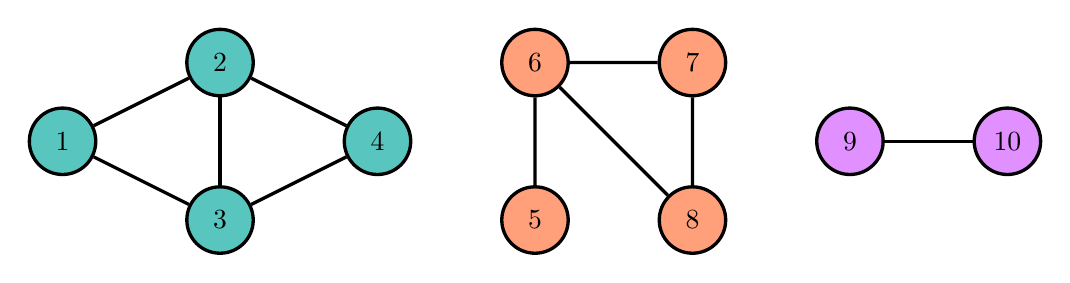
\begin{tikzpicture}[very thick,level/.style={sibling distance=70mm/#1}]
\draw (0, 0) node [vertex] (n1) {1};
\draw (2, 1) node [vertex] (n2) {2};
\draw (2, -1) node  [vertex] (n3) {3};
\draw (4, 0) node [vertex] (n4) {4};
\draw (n1) -- (n2);
\draw (n2) -- (n3);
\draw (n3) -- (n4);
\draw (n2) -- (n4);
\draw (n1) -- (n3);
\draw (6, -1) node [vertex, fill=mysalmon] (n5) {5};
\draw (6, 1) node [vertex, fill=mysalmon] (n6) {6};
\draw (8, 1) node [vertex, fill=mysalmon] (n7) {7};
\draw (8, -1) node [vertex, fill=mysalmon] (n8) {8};
\draw (n5) -- (n6) -- (n7) -- (n8) -- (n6);
\draw (10, 0) node[vertex, fill=mypurple] (n9) {9};
\draw (12, 0) node[vertex, fill=mypurple] (n10) {10};
\draw (n9) -- (n10);
\end{tikzpicture}
\end{center}

A \textit{strongly connected component} of a directed graph is a subgraph such that every vertex in the component can be reached from any other vertex in the component.

\begin{center}
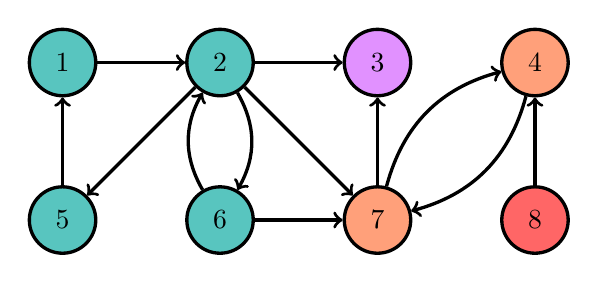
\begin{tikzpicture}[very thick,level/.style={sibling distance=70mm/#1}]
\draw (0, 0) node [vertex] (n1) {5};
\draw (2, 0) node [vertex] (n2) {6};
\draw (4, 0) node [vertex, fill=mysalmon] (n3) {7};
\draw (6, 0) node [vertex, fill=myred] (n4) {8};
\draw (0, 2) node [vertex] (m1) {1};
\draw (2, 2) node [vertex] (m2) {2};
\draw (4, 2) node [vertex, fill=mypurple] (m3) {3};
\draw (6, 2) node [vertex, fill=mysalmon] (m4) {4};
\draw[->] (m1) -- (m2);
\draw[->] (m2) -- (n1);
\draw[->] (n1) -- (m1);
\draw[->] (n2) edge [bend left] (m2);
\draw[->] (m2) edge [bend left] (n2);
\draw[->] (n2) -- (n3);
\draw[->] (m2) -- (m3);
\draw[->] (m2) -- (n3);
\draw[->] (n3) -- (m3);
\draw[->] (n3) edge [bend left] (m4);
\draw[->] (m4) edge [bend left] (n3);
\draw[->] (n4) -- (m4);
\end{tikzpicture}
\end{center}

Finding the connected components of an undirected graph is a straightforward problem, while finding the strongly connected components of a directed graph is more complicated.

\subsection{Flood Fill}

Really any kind of search method solves the undirected graph connected components problem. We could use recursion with a depth-first search. To avoid using the run-time stack, we could use a queue to perform a breadth-first search. Both of these run in $O(E+V)$ time. I would recommend in general to use the BFS.

\subsection{Union-Find (Disjoint Set Union)}

The union-find data structure is another way for us to solve the connected components problem. Union-find is unique from the other search techniques in that it can process input as it is presented, edge by edge. This also means it is possible to add more edges at the end, therefore changing the graph, while still running quickly. An algorithm that works like this is an \textit{online algorithm}, while an algorithm that requires all the input data presented at the beginning is an \textit{offline algorithm}.

A natural idea for solving the connected components problem is for each vertex to maintain a pointer to another vertex it's connected to, forming a \textit{forest}, or collection of trees. To check whether two elements are in the same component, simply trace the tree up to the root by jumping up each pointer.

\begin{center}
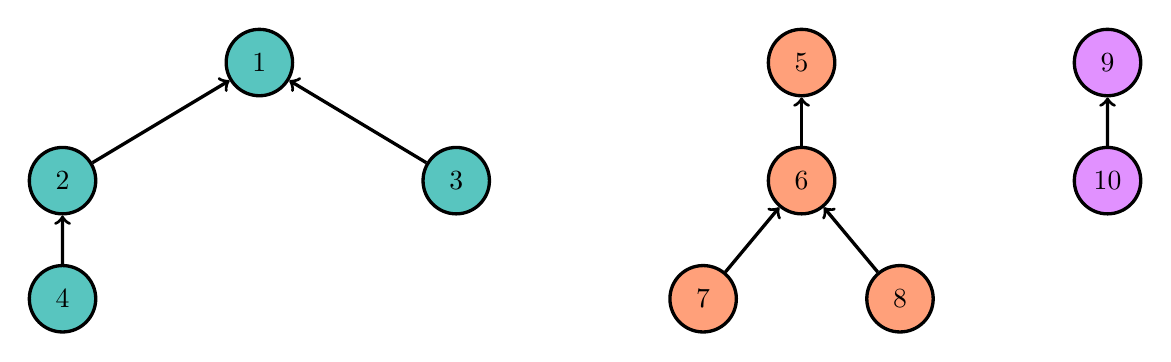
\begin{tikzpicture}[very thick,edge from parent/.style={draw,<-},level/.style={sibling distance=50mm/#1}]
\node [vertex, fill = mysalmon] (r2) {5}
  child {
      node [vertex, fill = mysalmon] {6}
      child { node [vertex, fill=mysalmon] {7} }
      child { node [vertex, fill=mysalmon] {8} }
  };

\node [vertex] [left=6cm of r2] (r1) {1}
  child {
    node [vertex] {2}
    child {
      node [vertex] {4}
    }
  }
  child {node [vertex] {3} };
  
\node [vertex, fill=mypurple] [right=3cm of r2] (r3) {9}
  child { node [vertex, fill=mypurple] {10} };
\end{tikzpicture}
\end{center}

The idea of a pointer can easily be stored within an array.

\begin{center}
{
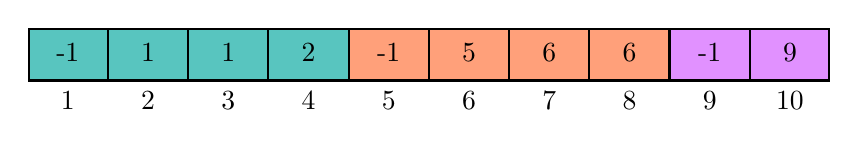
\begin{tikzpicture}[
  thick,
  myrect/.style={
    draw,
    rectangle split,
    rectangle split horizontal,
    rectangle split parts=#1,
    rectangle split part align=left,
    text width=5ex,
    text centered
    },
  mycallout/.style={
    shape=rectangle callout,
    rounded corners,
    fill=mysalmon,
    callout absolute pointer={#1},
    callout pointer width=1cm
  }  
]

\node[myrect=10, rectangle split part fill={myseagreen, myseagreen, myseagreen, myseagreen, mysalmon, mysalmon, mysalmon, mysalmon, mypurple, mypurple}]
  (array1)
  {
  					\strut -1
  \nodepart{two}	\strut 1
  \nodepart{three}	\strut 1
  \nodepart{four}	\strut 2
  \nodepart{five}	\strut -1
  \nodepart{six}	\strut 5
  \nodepart{seven}	\strut 6
  \nodepart{eight}	\strut 6
  \nodepart{nine}	\strut -1
  \nodepart{ten}	\strut 9
  };
\foreach \Valor [count=\Valori from 1] in {one ,two ,three ,four ,five ,six ,seven ,eight ,nine ,ten }
  \node[below] at (array1.\Valor south) {\Valori};

\end{tikzpicture}
}
\end{center}

We want to support two operations: $find(v)$, which returns the root of the tree containing $v$, and $union(u,v)$, which merges the components containing $u$ and $v$. This second operation is easy given the first; simply set the pointer of $find(u)$ to be $find(v)$.

$union(4, 6)$, unoptimized:

\begin{center}
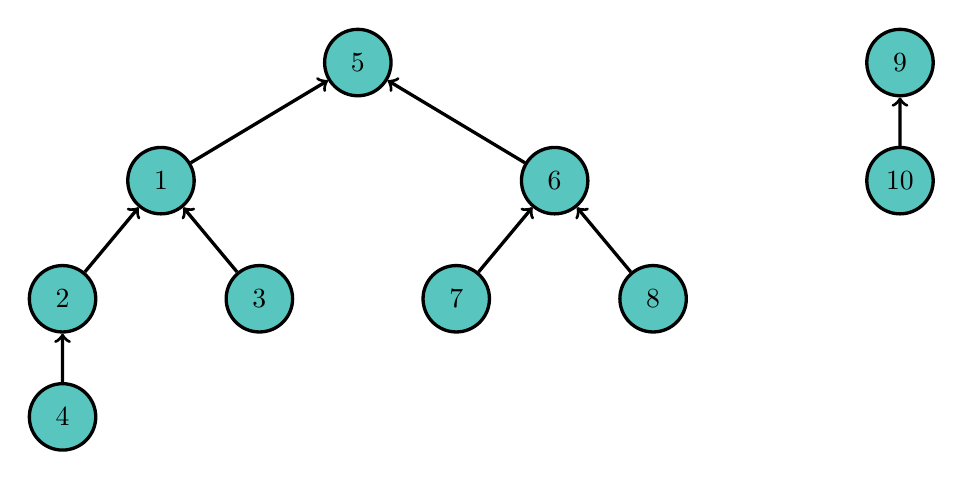
\begin{tikzpicture}[very thick,edge from parent/.style={draw,<-},level/.style={sibling distance=50mm/#1}]
\node [vertex] (r2) {5}
	child {
    node [vertex] (r1) {1}
	  child {
 	   node [vertex] {2}
  	  child {
   	   node [vertex] {4}
  	  }
	  }
 	 child {node [vertex] {3} }
  }
  child {
  node [vertex] {6}
		child { node [vertex] {7} }
   		child { node [vertex] {8} }
    };
\node [vertex] [right=6cm of r2] (r3) {9}
  child { node [vertex] {10} };
\end{tikzpicture}
\end{center}

A problem quickly arises -- the $find$ operation threatens to become linear. There are two simple things we can do to optimize this.

The first is to always add the shorter tree to the taller tree, as we want to minimize the maximum height. An easy heuristic for the height of the tree is simply the number of elements in that tree. We can keep track of the size of the tree with a second array. This heuristic is obviously not perfect, as a larger tree can be shorter than a smaller tree, but it turns out with our second optimization that this problem doesn't matter.

The second fix is to simply assign the pointer associated with $v$ to be $find(v)$ at the end of the $find$ operation. We can design $find(v)$ to recursively call $find$ on the pointer associated with $v$, so this fix sets pointers associated with nodes along the entire chain from $v$ to $find(v)$ to be $find(v)$. These two optimizations combined make the $union$ and $find$ operations $O(\alpha (V))$, where $\alpha(n)$ is the inverse Ackermann function, and for all practical values of $n$, $\alpha(n) < 5$.

$find(4)$, optimized:

\begin{center}
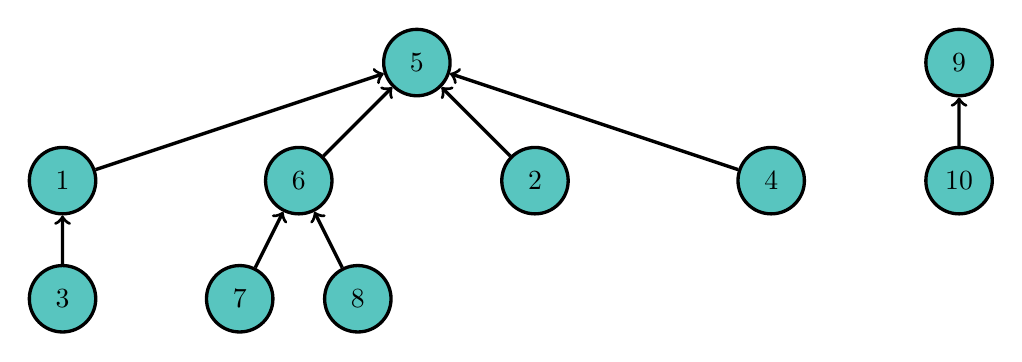
\begin{tikzpicture}[very thick,edge from parent/.style={draw,<-},level/.style={sibling distance=30mm/#1}]
\node [vertex] (r2) {5}
	child {
    node [vertex] (r1) {1}
 	 child {node [vertex] {3} }
  }
  child {
  node [vertex] {6}
		child { node [vertex] {7} }
   		child { node [vertex] {8} }
    }
  child {node[vertex] {2}}
  child {node[vertex] {4}};
\node [vertex] [right=6cm of r2] (r3) {9}
  child { node [vertex] {10} };
\end{tikzpicture}
\end{center}

\begin{algorithm}[H]
\caption{Union-Find}
%\label{}
\begin{algorithmic}
\Function{Find}{$v$}
	\If {$v$ is the root}
		\State \Return $v$
    \EndIf
    \State $parent(v) \gets \Call{Find}{parent(v)}$
    \State \Return $parent(v)$
\EndFunction
\Function{Union}{$u$, $v$}
	\State $uRoot \gets \Call{Find}{u}$
	\State $vRoot \gets \Call{Find}{v}$
    \If {$uRoot = vRoot$}
		\State \Return
	\EndIf
    \If {$size(uRoot)<size(vRoot)$}
    	\State $parent(uRoot) \gets vRoot$
        \State $size(vRoot) \gets size(uRoot) + size(vRoot)$
    \Else
    	\State $parent(vRoot) \gets uRoot$
        \State $size(uRoot) \gets size(uRoot) + size(vRoot)$
    \EndIf
\EndFunction
\end{algorithmic}
\end{algorithm}

\subsection{Tarjan}

Tarjan's algorithm for strongly connected components

\section{Shortest Path}

A classic. Assign nonnegative weights to each of the edges, where the weight of the edge $(u,v)$ represents the distance from $u$ to $v$. This graph can be either directed or undirected.

\subsection{Dijkstra}

Dijkstra's algorithm solves the single-source shortest path problem. From any vertex, we can compute the shortest path to each of the remaining vertices in the graph. The two formulations of Dijkstra's algorithm run in $O(V^2)$ or $O(E\log{V})$ time, whichever one suits us better. Note that it is possible to do better than $O(E\log{V})$ using a Fibonacci heap. The former works nicely on dense graphs, as $E \approx V^2$, while the latter works better on sparse graphs, as $E \approx V$.

For every vertex $v$ in the graph, we keep track of the shortest known distance $dist(v)$ from the source to $v$, a boolean $visited(v)$ to keep track of which nodes we ``visited,'' and a pointer to the previous node in the shortest known path $prev(v)$ so that we can trace the shortest path once the algorithm finishes.

Dijkstra iteratively ``visits'' the next nearest vertex, updating the distances to that vertex's neighbors if necessary. Therefore, at any step, we have the first however-many nearest vertices to the source, which we call ``visited'' and for which the shortest path is known. We also have the shortest path to all the remaining vertices that stays within the ``visited'' vertices besides for the very last edge, if such a path exists. We claim that the known distance to the closest vertex that has not yet been visited is the shortest distance. We can then ``visit'' that vertex. It shouldn't be hard to prove that this algorithm indeed calculates the shortest path.

The $O(V^2)$ implementation immediately follows.

\begin{algorithm}[H]
\caption{Dijkstra}
\begin{algorithmic}
\ForAll{vertices $v$}
	\State $dist(v) \gets \infty$
	\State $visited(v) \gets 0$
    \State $prev(v) \gets -1$
\EndFor
\State $dist(src) \gets 0$
\While{$\exists v$ s.t. $visited(v)=0$}
	\State $v \equiv v$ s.t. $visited(v)=0$ with min $dist(v)$
    \State $visited(v) \gets 1$
	\ForAll{neighbors $u$ of $v$}
    	\If{$visited(u) = 0$}
    		\State $alt \gets dist(v) + weight(v, u)$
			\If{$alt < dist(u)$}
				\State $dist(u) \gets alt$
   	        	\State $prev(u) \gets v$
			\EndIf
        \EndIf
    \EndFor
\EndWhile
\end{algorithmic}
\end{algorithm}

\begin{center}
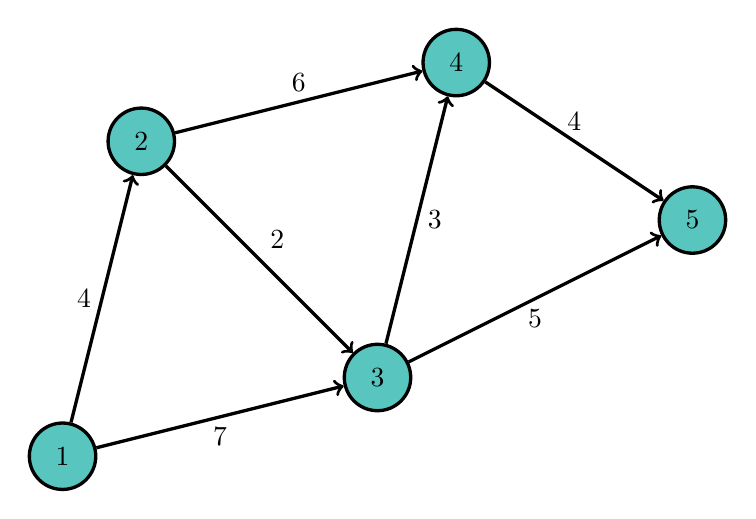
\begin{tikzpicture}[very thick,edge from parent/.style={draw,<-},level/.style={sibling distance=30mm/#1}]
\draw (0, 0) node [vertex] (v1) {1};
\draw (1, 4) node [vertex] (v2) {2};
\draw (4, 1) node [vertex] (v3) {3};
\draw (5, 5) node [vertex] (v4) {4};
\draw (8, 3) node [vertex] (v5) {5};
\draw[->] (v1) -- (v2) node[midway, left] {4};
\draw[->] (v2) -- (v3) node[midway, above right] {2};
\draw[->] (v1) -- (v3) node[midway, below] {7};
\draw[->] (v2) -- (v4) node[midway, above] {6};
\draw[->] (v3) -- (v4) node[midway, right] {3};
\draw[->] (v3) -- (v5) node[midway, below] {5};
\draw[->] (v4) -- (v5) node[midway, above] {4};
\end{tikzpicture}
\end{center}

Let's run Dijkstra's algorithm on the above graph with vertex 1 as the source. We first set all the distances besides the source to be $\infty$.

\begin{center}
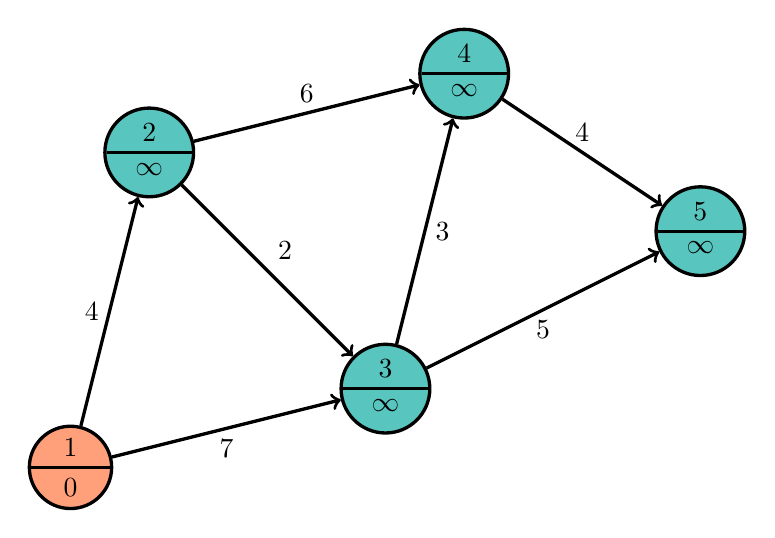
\begin{tikzpicture}[very thick,edge from parent/.style={draw,<-},level/.style={sibling distance=30mm/#1}]
\draw (0, 0) node [splitvertex, fill=mysalmon] (v1) {1\nodepart{lower}0};
\draw (1, 4) node [splitvertex] (v2) {2\nodepart{lower}$\infty$};
\draw (4, 1) node [splitvertex] (v3) {3\nodepart{lower}$\infty$};
\draw (5, 5) node [splitvertex] (v4) {4\nodepart{lower}$\infty$};
\draw (8, 3) node [splitvertex] (v5) {5\nodepart{lower}$\infty$};
\draw[->] (v1) -- (v2) node[midway, left] {4};
\draw[->] (v2) -- (v3) node[midway, above right] {2};
\draw[->] (v1) -- (v3) node[midway, below] {7};
\draw[->] (v2) -- (v4) node[midway, above] {6};
\draw[->] (v3) -- (v4) node[midway, right] {3};
\draw[->] (v3) -- (v5) node[midway, below] {5};
\draw[->] (v4) -- (v5) node[midway, above] {4};
\end{tikzpicture}
\end{center}

Now, we continue choosing the closest unvisited node, mark it as visited, and and update its neighbors.

\begin{center}
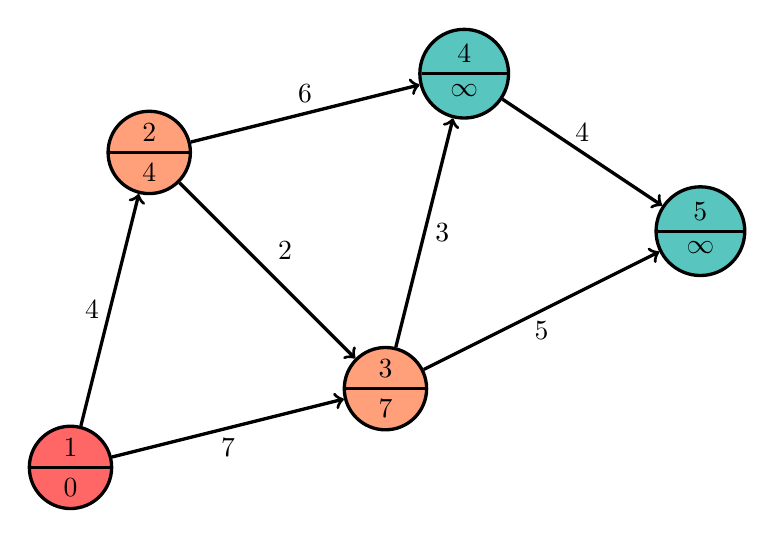
\begin{tikzpicture}[very thick,edge from parent/.style={draw,<-},level/.style={sibling distance=30mm/#1}]
\draw (0, 0) node [splitvertex, fill=myred] (v1) {1\nodepart{lower}0};
\draw (1, 4) node [splitvertex, fill=mysalmon] (v2) {2\nodepart{lower}4};
\draw (4, 1) node [splitvertex, fill=mysalmon] (v3) {3\nodepart{lower}7};
\draw (5, 5) node [splitvertex] (v4) {4\nodepart{lower}$\infty$};
\draw (8, 3) node [splitvertex] (v5) {5\nodepart{lower}$\infty$};
\draw[->] (v1) -- (v2) node[midway, left] {4};
\draw[->] (v2) -- (v3) node[midway, above right] {2};
\draw[->] (v1) -- (v3) node[midway, below] {7};
\draw[->] (v2) -- (v4) node[midway, above] {6};
\draw[->] (v3) -- (v4) node[midway, right] {3};
\draw[->] (v3) -- (v5) node[midway, below] {5};
\draw[->] (v4) -- (v5) node[midway, above] {4};
\end{tikzpicture}
\end{center}

\begin{center}
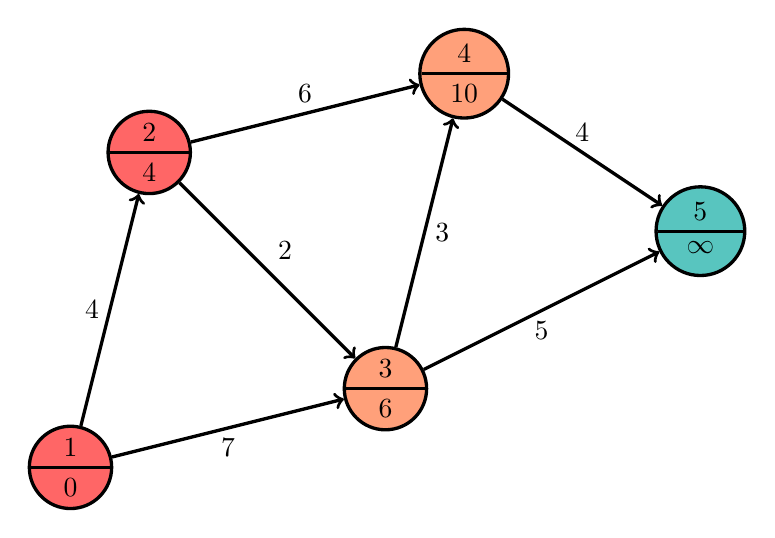
\begin{tikzpicture}[very thick,edge from parent/.style={draw,<-},level/.style={sibling distance=30mm/#1}]
\draw (0, 0) node [splitvertex, fill=myred] (v1) {1\nodepart{lower}0};
\draw (1, 4) node [splitvertex, fill=myred] (v2) {2\nodepart{lower}4};
\draw (4, 1) node [splitvertex, fill=mysalmon] (v3) {3\nodepart{lower}6};
\draw (5, 5) node [splitvertex, fill=mysalmon] (v4) {4\nodepart{lower}10};
\draw (8, 3) node [splitvertex] (v5) {5\nodepart{lower}$\infty$};
\draw[->] (v1) -- (v2) node[midway, left] {4};
\draw[->] (v2) -- (v3) node[midway, above right] {2};
\draw[->] (v1) -- (v3) node[midway, below] {7};
\draw[->] (v2) -- (v4) node[midway, above] {6};
\draw[->] (v3) -- (v4) node[midway, right] {3};
\draw[->] (v3) -- (v5) node[midway, below] {5};
\draw[->] (v4) -- (v5) node[midway, above] {4};
\end{tikzpicture}
\end{center}

\begin{center}
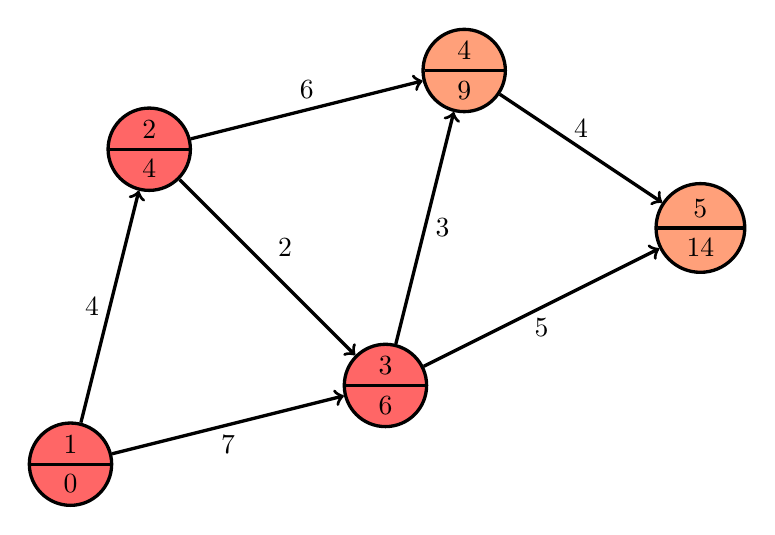
\begin{tikzpicture}[very thick,edge from parent/.style={draw,<-},level/.style={sibling distance=30mm/#1}]
\draw (0, 0) node [splitvertex, fill=myred] (v1) {1\nodepart{lower}0};
\draw (1, 4) node [splitvertex, fill=myred] (v2) {2\nodepart{lower}4};
\draw (4, 1) node [splitvertex, fill=myred] (v3) {3\nodepart{lower}6};
\draw (5, 5) node [splitvertex, fill=mysalmon] (v4) {4\nodepart{lower}9};
\draw (8, 3) node [splitvertex, fill=mysalmon] (v5) {5\nodepart{lower}14};
\draw[->] (v1) -- (v2) node[midway, left] {4};
\draw[->] (v2) -- (v3) node[midway, above right] {2};
\draw[->] (v1) -- (v3) node[midway, below] {7};
\draw[->] (v2) -- (v4) node[midway, above] {6};
\draw[->] (v3) -- (v4) node[midway, right] {3};
\draw[->] (v3) -- (v5) node[midway, below] {5};
\draw[->] (v4) -- (v5) node[midway, above] {4};
\end{tikzpicture}
\end{center}

\begin{center}
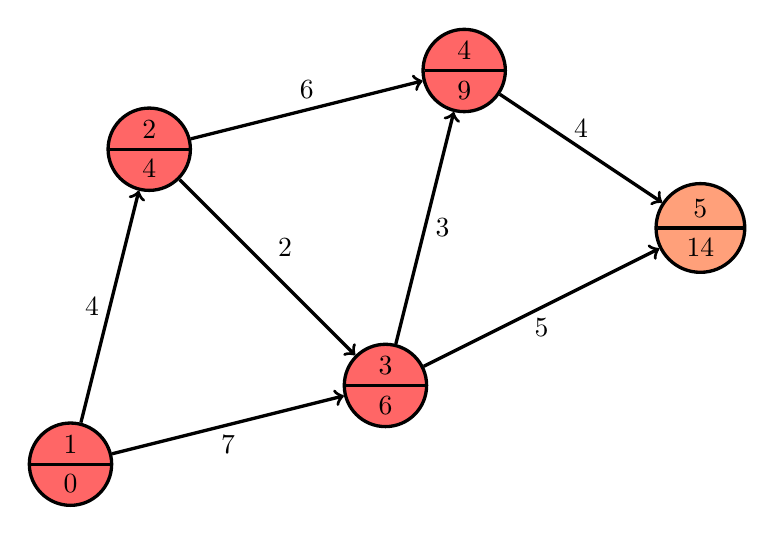
\begin{tikzpicture}[very thick,edge from parent/.style={draw,<-},level/.style={sibling distance=30mm/#1}]
\draw (0, 0) node [splitvertex, fill=myred] (v1) {1\nodepart{lower}0};
\draw (1, 4) node [splitvertex, fill=myred] (v2) {2\nodepart{lower}4};
\draw (4, 1) node [splitvertex, fill=myred] (v3) {3\nodepart{lower}6};
\draw (5, 5) node [splitvertex, fill=myred] (v4) {4\nodepart{lower}9};
\draw (8, 3) node [splitvertex, fill=mysalmon] (v5) {5\nodepart{lower}14};
\draw[->] (v1) -- (v2) node[midway, left] {4};
\draw[->] (v2) -- (v3) node[midway, above right] {2};
\draw[->] (v1) -- (v3) node[midway, below] {7};
\draw[->] (v2) -- (v4) node[midway, above] {6};
\draw[->] (v3) -- (v4) node[midway, right] {3};
\draw[->] (v3) -- (v5) node[midway, below] {5};
\draw[->] (v4) -- (v5) node[midway, above] {4};
\end{tikzpicture}
\end{center}

\begin{center}
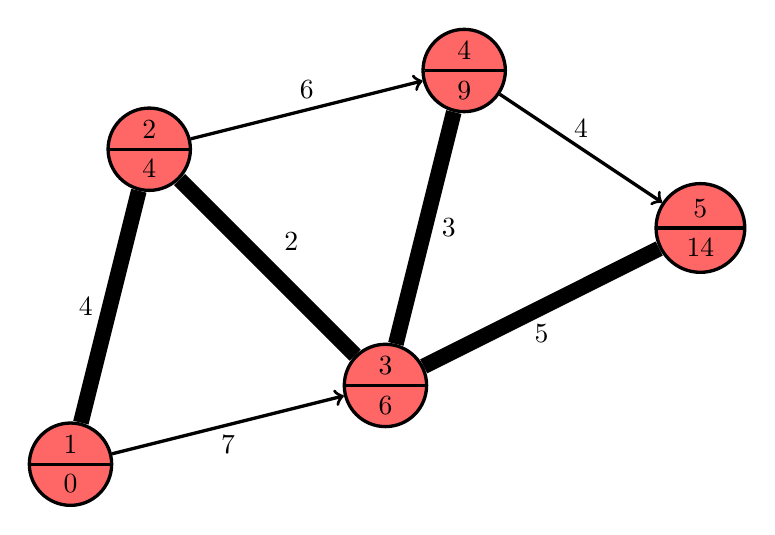
\begin{tikzpicture}[very thick,edge from parent/.style={draw,<-},level/.style={sibling distance=30mm/#1}]
\draw (0, 0) node [splitvertex, fill=myred] (v1) {1\nodepart{lower}0};
\draw (1, 4) node [splitvertex, fill=myred] (v2) {2\nodepart{lower}4};
\draw (4, 1) node [splitvertex, fill=myred] (v3) {3\nodepart{lower}6};
\draw (5, 5) node [splitvertex, fill=myred] (v4) {4\nodepart{lower}9};
\draw (8, 3) node [splitvertex, fill=myred] (v5) {5\nodepart{lower}14};
\draw[line width=2mm] (v1) -- (v2) node[midway, left] {4};
\draw[line width=2mm] (v2) -- (v3) node[midway, above right] {2};
\draw[->] (v1) -- (v3) node[midway, below] {7};
\draw[->] (v2) -- (v4) node[midway, above] {6};
\draw[line width=2mm] (v3) -- (v4) node[midway, right] {3};
\draw[line width=2mm] (v3) -- (v5) node[midway, below] {5};
\draw[->] (v4) -- (v5) node[midway, above] {4};
\end{tikzpicture}
\end{center}

The slow part of the $O(V^2)$ formulation is the linear search for the vertex $v$ with the minimum $dist(v)$. We happen to have a data structure that resolves this problem -- a binary heap. The main problem with using the standard library heap is having repeated vertices in the heap. We could just ignore this problem and discard visited vertices as they come out of the heap. Alternatively, we could choose never to have repeated vertices in the heap. To do this, we need to be able to change the value of the distances once they are already in the heap, or \textit{decrease-key}. This is a pretty simple function to add, however, if you have a heap already coded. Either way, we achieve $O(E \log{V})$, as we do $E+V$ updates to our heap, each costing $O(V)$.

\subsection{Floyd-Warshall}

Dijkstra is nice when we are dealing with edges with nonnegative weights and are looking for the distances from one vertex to all the others. Floyd-Warshall solves the shortest path problem for all pairs of vertices in $O(V^3)$ time, which is faster than $V$ single-source Dijkstra runs on a dense graph. Floyd-Warshall works even if some edge weights are negative but not if the graph has a negative cycle.

\begin{algorithm}[H]
\caption{Floyd-Warshall}
\begin{algorithmic}
\ForAll{vertices $v$}
	\State $dist(v,v)=0$
\EndFor
\ForAll{edges $(u,v)$}
	\State $dist(u,v)=weight(u,v)$
\EndFor
\ForAll{vertices $k$}
	\ForAll{vertices $i$}
    	\ForAll{vertices $j$}
        	\If{$dist(i,j) > dist(i,k)+dist(k,j)$}
            	\State $dist(i,j) \gets dist(i,k)+dist(k,j)$
            \EndIf
        \EndFor
    \EndFor
\EndFor
\end{algorithmic}
\end{algorithm}

\subsection{Bellman-Ford}

Bellman-Ford is a single-source $O(VE)$ shortest path algorithm that works when edge weights can be negative. It is preferable to Floyd-Warshall when the graph is sparse and we only need the answer for one source. Like Floyd-Warshall, the algorithm fails if the graph contains a negative cycle, but the algorithm is still useful for detecting negative cycles.

The idea here is the shortest path, assuming no negative cycles, has length at most $V-1$.

\begin{algorithm}[H]
\caption{Bellman-Ford}
\begin{algorithmic}
\ForAll{vertices $v$}
	\State $dist(v)\gets\infty$
    \State $prev(v)=\gets -1$
\EndFor
\State $dist(src) \gets 0$
\For{$i\equiv 1,V-1$}
	\ForAll{edges $(u,v)$}
		\If{$dist(u)+weight(u,v) < dist(v)$}
    	    \State $dist(v) \gets dist(u)+weight(u,v)$
	        \State $prev(v) \gets u$
        \EndIf
	\EndFor
\EndFor
\ForAll{edges $(u,v)$}
	\Comment{check for negative cycles}
	\If{$dist(u)+weight(u,v) < dist(v)$}
   	    \State{negative cycle detected}
	\EndIf
\EndFor
\end{algorithmic}
\end{algorithm}

\section{Minimum Spanning Tree}

Consider a connected, undirected graph. A \textit{spanning tree} is a subgraph that is a tree and contains every vertex in the original graph. A \textit{minimum spanning tree} is a spanning tree such that the sum of the edge weights of the tree is minimized. Finding the minimum spanning tree uses many of the same ideas discussed earlier.

\begin{center}
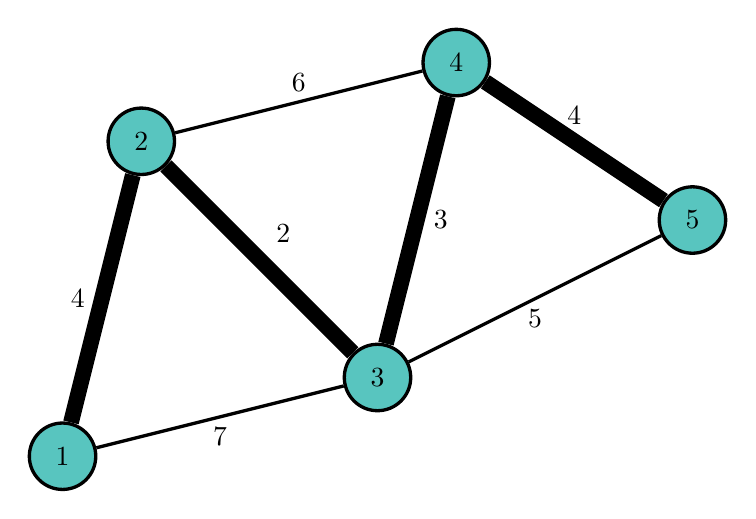
\begin{tikzpicture}[very thick,edge from parent/.style={draw,<-},level/.style={sibling distance=30mm/#1}]
\draw (0, 0) node [vertex] (v1) {1};
\draw (1, 4) node [vertex] (v2) {2};
\draw (4, 1) node [vertex] (v3) {3};
\draw (5, 5) node [vertex] (v4) {4};
\draw (8, 3) node [vertex] (v5) {5};
\draw[line width=2mm] (v1) -- (v2) node[midway, left] {4};
\draw[line width=2mm] (v2) -- (v3) node[midway, above right] {2};
\draw (v1) -- (v3) node[midway, below] {7};
\draw (v2) -- (v4) node[midway, above] {6};
\draw[line width=2mm] (v3) -- (v4) node[midway, right] {3};
\draw (v3) -- (v5) node[midway, below] {5};
\draw[line width=2mm] (v4) -- (v5) node[midway, above] {4};
\end{tikzpicture}
\end{center}

\subsection{Prim}

Prim's algorithm for finding the minimum spanning tree is very similar to Dijkstra's algorithm for finding the shortest path. Like Dijkstra, it iteratively adds a new vertex at a time to build a tree. The only difference is $dist(v)$ stores the shortest distance from \textit{any} visited node instead of the source.

\begin{algorithm}[H]
\caption{Prim}
\begin{algorithmic}
\ForAll{vertices $v$}
	\State $dist(v) \gets \infty$
	\State $visited(v) \gets 0$
    \State $prev(v) \gets -1$
\EndFor
\State $dist(src) \gets 0$
\While{$\exists v$ s.t. $visited(v)=0$}
	\State $v \equiv v$ s.t. $visited(v)=0$ with min $dist(v)$
    \State $visited(v) \gets 1$
	\ForAll{neighbors $u$ of $v$}
    	\If{$visited(u) = 0$}
			\If{$weight(v, u) < dist(u)$}
				\State $dist(u) \gets weight(v, u)$
   	        	\State $prev(u) \gets v$
			\EndIf
        \EndIf
    \EndFor
\EndWhile
\end{algorithmic}
\end{algorithm}

The proof of correctness is left as an exercise. The complexity of this algorithm depends on how the minimum unvisited vertex is calculated. Using the same approaches as Dijkstra, we can achieve $O(V^2)$ or $O(E \log{V})$.

\subsection{Kruskal}

While Prim greedily adds vertices to the tree, Kruskal's algorithm greedily adds edges. It iterates over all the edges, sorted by weight. We need to watch out for adding a cycle, breaking the tree structure, which means we need to keep track of each vertex's connected component. If an edge connects two vertices from the same connected component, we don't want to add it to our tree. However, we have a union-find algorithm that works perfectly for this.

\begin{algorithm}[H]
\caption{Kruskal}
\begin{algorithmic}
\ForAll{edges $(u,v)$ in sorted order}
	\If{$\Call{Find}{u} \not= \Call{Find}{v}$}
		\State add $(u,v)$ to spanning tree
		\State $\Call{Union}{u,v}$
	\EndIf
\EndFor
\end{algorithmic}
\end{algorithm}

This algorithm requires a sort of the edges and thus has complexity $O(E \log{E}) = O(E \log{V})$.

\section{Eulerian Tour}

An \textit{Eulerian tour} of a graph is a path that traverses every edge exactly once. If the tour ends exactly where it started, it is called an \textit{Eulerian circuit}. A graph has an Eulerian circuit if it is connected and every vertex has even degree. A graph has an Eulerian path if it is connected and all vertices but exactly two have even degrees. The mathematical proofs for these graph properties hinge on the idea that removing a cycle from the graph maintains the Eulerian property. We construct an Eulerian tour by appealing to this idea.

\begin{algorithm}[H]
\caption{Eulerian Tour}
\begin{algorithmic}
\Function{FindTour}{$v$}
\While{$v$ has a neighbor $u$}
	\State delete edge $(v,u)$
	\State \Call{FindTour}{$u$}
	\Comment{\Call{FindTour}{$u$} must trace a circuit back to $v$}
\EndWhile
\State add $v$ to tour
\EndFunction
\end{algorithmic}
\end{algorithm}

It is not preferable to use the run-time stack; we can use our own stack if necessary.

If the graph contains an Eulerian circuit, we call this function on any vertex we like. If it contains an Eulerian path, we call this function on one of the vertices with odd degree.

\section{Maximum Flow}

We are given a directed graph with weighted edges, a source node, and a sink node. A \textit{flow} is sent from the source to the sink. Each edge weight represents the maximum capacity of that edge. For every node besides the source and the sink node, total flow in is equal to total flow out. We can think of a flow network as a series of pipes through which water travels from an entrance to an exit in the network. The edge capacities represent pipe thickness. At any node, the total rate at which water enters the node must equal the total rate at which it exits the node, and along any path, the rate at which water flows is bottlenecked by the thinnest pipe.

More formally, for a graph $G(V,E)$, where $c(u,v)$ represents the capacity of the edge from $u$ to $v$, the flow $f(u,v)$ from a source $s$ to a sink $t$ satisfies

\begin{align*}
f(u,v) &\le c(u,v) \forall (u,v) \in E \\
f(u,v) &= -f(v,u) \forall (u,v) \in E \\
\sum_{v \in V} f(u,v) &= 0 \forall u \in V \setminus \{s,t\} \\
\sum_{v \in V} f(s,v) &= \sum_{v \in V} f(v,t) = |f|,
\end{align*}

where $|f|$ represents the total flow from the source to the sink.

A \textit{maximum flow} is one that maximizes the total flow $|f|$ from $s$ to $t$, or in our example, maximizes the rate at which water can flow through our network.

We'll also define the residual capacity $c_f(u,v) = c(u,v) - f(u,v)$. Note that $c_f(u,v) \ge 0$ by the conditions imposed on $f$. The residual capacity of an edge represents how much capacity is left after a certain amount of flow has already been sent. We therefore have the residual graph $G_f(V,E_f)$, where $E_f$ is the graph of residual edges, or all edges $(u,v) \in V^2$ satisfying $c_f(u,v) > 0$.

A natural approach to ``solving'' this problem would be to simply greedily add flow.

Find a path from the source to the sink in which all the edges have positive weight in the residual graph. Send flow along this path; that is, find the max flow across this path, which is the minimum weight of any edge on this particular path. Call this value $cap$. Then subtract $cap$ from the residual capacity of every edge in the path. We repeat, and this is guaranteed to terminate since on any given move, we remove an edge from our residual graph.

What is wrong with our greedy approach? Consider the following graph:

\begin{center}
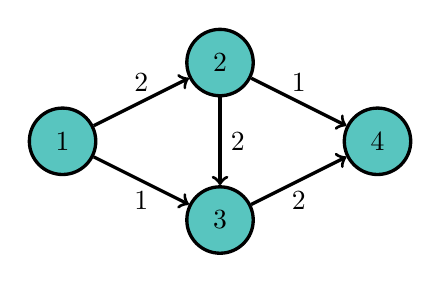
\begin{tikzpicture}[very thick,level/.style={sibling distance=70mm/#1}]
\draw (0, 0) node [vertex] (n1) {1};
\draw (2, 1) node [vertex] (n2) {2};
\draw (2, -1) node  [vertex] (n3) {3};
\draw (4, 0) node [vertex] (n4) {4};
\draw[->] (n1) -- (n2) node[midway, above] {2};
\draw[->] (n2) -- (n3) node[midway, right] {2};
\draw[->] (n3) -- (n4) node[midway, below] {2};
\draw[->] (n2) -- (n4) node[midway, above] {1};
\draw[->] (n1) -- (n3) node[midway, below] {1};
\end{tikzpicture}
\end{center}

The max flow from vertex 1 to vertex 4 is 3, but greedy gives only 2. This is because the best possible single path from the source to the sink may not be included the best possible overall flow.

\subsection{Ford-Fulkerson}

We somehow need a way to fix the inclusion of any suboptimal paths in our greedy approach, or to ``send flow back'' in case we sent it through a suboptimal path. We do this by introducing the \textit{reverse edge} to our residual graph.

Find a path from the source to the sink in which all the edges have positive weight in the residual graph. Find the max flow across this path, which is the minimum weight of any edge on this particular path. Call this value $cap$. Then subtract $cap$ from the residual capacity of every edge along the path and \textit{increment the residual capacity of the reverse edge} (the edge connecting the same two vertices but running in the opposite direction) by $cap$. We call this operation on the path \textit{augmenting the path}. We simply choose an augmenting path until no such paths exist.

\begin{algorithm}[H]
\caption{Ford-Fulkerson}
\begin{algorithmic}
\Function{AugmentPath}{path $p=\{v_i\}_{i=1}^m$, where $(v_i,v_{i+1}) \in E_f$, $v_1=s$, $v_m=t$}
\State $cap \gets \min_{i=1}^{m-1}(c_f(v_i,v_{i+1}))$
\For{$i \equiv 1, m-1$}
	\State $f(v_i,v_{i+1}) \gets f(v_i,v_{i+1}) + cap$
	\State $c_f(v_i,v_{i+1}) \gets c_f(v_i,v_{i+1}) + cap$
	\State $f(v_{i+1},v_i) \gets f(v_{i+1},v_i) - cap$
	\State $c_f(v_{i+1},v_i) \gets c_f(v_{i+1},v_i) + cap$
	\Comment incrementing reverse edge
\EndFor
\EndFunction
\Function{MaxFlow}{$G(V,E)$, $s,t \in V$}
	\ForAll{$(u,v) \in V^2$}
		\State $f(u,v) \gets 0$
		\State $c_f(u,v) \gets c(u,v)$
	\EndFor
	\State $|f| \gets 0$
	\While{$\exists p=\{v_i\}_{i=1}^m$, where $(v_i,v_{i+1}) \in E_f$, $v_1=s$, $v_m=t$}
		\State $cap \gets \min_{i=1}^{m-1}(c_f(v_i,v_{i+1}))$
		\State $|f| \gets |f| + cap$
		\State \Call{AugmentPath}{$p$}
	\EndWhile
	\Return $|f|$
\EndFunction
\end{algorithmic}
\end{algorithm}

The difference between this algorithm and the greedy approach from earlier is that the paths we now allow may run along a reverse path, essentially undoing any suboptimal flow from earlier. These more general paths in our residual graph are called \textit{augmenting paths}.

This algorithm is guaranteed to terminate for graphs with integral weights. Its performance is bounded by $O(Ef)$, where $f$ is the maximum flow and $E$ is the number of edges, as finding a path from $s$ to $t$ takes $O(E)$ and increments the total flow $f$ by at least 1. The concept of removing edges can't be used to produce a stricter bound because while an edge in one direction may be removed from the residual graph, doing so creates an edge in the other direction.

In its crudest form, Ford-Fulkerson does not specify on which path to push flow if multiple paths exist. It simply states that as long as such a path exists, push flow onto it. In addition to being slow, Ford-Fulkerson, as it is stated, is not guaranteed to terminate for graphs with non-integral capacities. In fact, it might not even converge to the maximum flow for irrational capacities. However, these problems can be fixed by simply specifying how the algorithm chooses the next path on which to push flow. Nonetheless, the Ford-Fulkerson algorithm is formulated beautifully mathematically and such is useful from a math perspective, as we will see with the Max-Flow Min-Cut Theorem.

\subsection{Max-Flow Min-Cut Theorem}

On a graph $G(V,E)$, an \textit{s-t cut} $C=(S,T)$ splits the partitions $V$ into $S$ and $T$ satisfying $s \in S$ and $t \in T$. The \textit{cut-set} of $C$ is the set of edges $\{(u,v) \in E : u \in S, v \in T\}$. The \textit{capacity} of an s-t cut is given by

\[c(S,T) = \sum_{(u,v) \in S \times T}c(u,v).\]

A \textit{minimum cut} is an s-t cut that minimizes $c(S,T)$.

A cut represents a set of edges that, once removed, separates $s$ from $t$. A minimum cut is therefore a set of edges that does this but minimizes the total capacity of the edges necessary to disconnect $s$ from $t$.

The max-flow min-cut theorem states that the maximum value of any s-t flow is equal to the minimum capacity of any s-t cut.

First, the capacity of any cut must be at least the total flow. This is true by contradiction. Any path from $s$ to $t$ has an edge in the cut-set, so therefore any flow from $s$ to $t$ is upper bounded by the capacity of the cut. Therefore, we need only construct one flow and one cut such that the capacity of the cut is equal to the flow.

We consider the residual graph $G_f$ produced at the completion of the Ford-Fulkerson augmenting path algorithm.\footnote{If you're concerned that the Ford-Fulkerson algorithm will never terminate, there always exists a sequence of paths chosen such that it will. Edmonds-Karp is one example that always terminates.} Let the set $S$ be all nodes reachable from $s$ and $T$ be $V \setminus S$. We wish to show that $C=(S,T)$ is a cut satisfying $|f|=c(S,T)=\sum_{(u,v) \in S \times T} c(u,v)$. This is true when the following is satisfied:

\begin{enumerate}

\item
All edges $(u,v) \in S \times T$ are fully saturated by the flow. That is, $c_f(u,v) = 0$.

\item
All reverse edges $(v, u) \in T \times S$ have zero flow. That is, $f(v,u) = 0$, or $c_f(v,u) = c(v,u)$.

\end{enumerate}

The first condition is true by the way we constructed $S$ and $T$, as if there existed a $(u,v)$ where $c_f(u,v) > 0$, then $v$ is accessible to $s$ and ought to have been in $S$.

The second condition is true by the way the Ford-Fulkerson algorithm constructed reverse edges. If net flow was sent from $v$ to $u$, then a reverse edge was constructed from $u$ to $v$, so again, $v$ is accessible to $s$, which is a contradiction.

Therefore, we have the flow
\[|f|=\sum_{(u,v) \in S \times T} c(u,v) - \sum_{(v,u) \in T \times S} 0 = c(S,T),\]
so we constructed a flow and a cut such that the flow $|f|$ is equal to the cut capacity $c(S,T)$, and we are done.

\subsection{Edmonds-Karp}

Edmonds-Karp is a refinement of Ford-Fulkerson. As stated earlier, Ford-Fulkerson is limited by not specifying on which path to push flow. There are many algorithms that resolve this issue in different ways; Edmonds-Karp fixes this by simply choosing the augmenting path of shortest unweighted length. This can be done easily using a BFS.

\begin{algorithm}[H]
\caption{Edmonds-Karp}
\begin{algorithmic}
\Function{ChoosePath}{$G_f(V,E_f)$, $s,t \in V$}
	\Comment{BFS}
	\State $visited(v)$ denotes $v$ has been added to queue
	\State $prev(v)$ denotes vertex preceding $v$ in BFS
	\State push $s$ on queue $q$
	\State $visited(s) \gets 1$
	\While{$q$ is not empty}
		\State $u \gets $ top of $q$
		\ForAll{neighbors $v$ of $u$ in $G_f$ where $visited(v)=0$}
			\State push $v$ on $q$
			\State $visited(v) \gets 1$
			\State $prev(v) \gets u$
		\EndFor
	\EndWhile
	\State pointer $curr \gets t$
	\While{$curr \not= s$}
		\State add $curr$ to beginning of path $p$
		\State $curr \gets prev(curr)$
	\EndWhile
	\State add $s$ to beginning of $p$
	\State \Return $p$
\EndFunction
\Function{MaxFlow}{$G(V,E)$, $s,t \in V$}
	\ForAll{$(u,v) \in V^2$}
		\State $f(u,v) \gets 0$
		\State $c_f(u,v) \gets c(u,v)$
	\EndFor
	\State $|f| \gets 0$
	\While{$t$ can be reached from $s$}
		\State $p \gets \Call{ChoosePath}{G_f,s,t}$
		\State $cap \gets \min_{i=1}^{m-1}(c_f(v_i,v_{i+1}))$
		\State $|f| \gets |f| + cap$
		\State \Call{AugmentPath}{$p$}
	\EndWhile
	\Return $|f|$
\EndFunction
\end{algorithmic}
\end{algorithm}

The BFS is clearly $O(E)$. To complete our analysis, we must somehow bound the number of times we need to perform the BFS. To do this, we'll look at what pushing flow on a path does to our residual graph; in particular, how it affects our BFS traversal tree. Note that each vertex is on some level $i$ in the BFS tree, characterized by the distance from the source $s$. For example, $L_0 = \{s\}$, $L_1$ contains all the neighbors of $s$, $L_2$ contains neighbors of neighbors not in $L_0$ or $L_1$, and so on.

We first claim that the level of any vertex in the graph is nondecreasing following an augment on a path $p$. If the augment saturates an edge, it may remove it from $G_f$, which cannot decrease the distance of any vertex from $s$. If the augment creates an edge $e=(u,v)$, that means we sent flow from $v$ to $u$ on the path $p$. Therefore, if $v$ was originally level $i$, $u$ must have been level $i+1$. The level of $u$ does not change by adding $(u,v)$, and the level of $v$ can either be $i$ or $i+2$, depending on whether edge $(v,u)$ was deleted in the process. Either way, the level of all vertices is nondecreasing.

Now consider the bottleneck edge $e=(u,v)$ of an augmenting path $p$, where the level of $u$ is $i$ and the level of $v$ is $i+1$. The push operation deletes the edge $e$, but the level of $v$ must stay at least $i+1$. Now for the edge $e$ to reappear in the graph $G_f$, flow must have been sent on the reverse edge $e'=(v,u)$ on some augmenting path $p'$. But on path $p'$, $u$ comes after $v$, which must be at least level $i+1$. Therefore, $u$ must be at least level $i$. But since the maximum level of a node that is connected to $s$ is $V-1$, an edge $e$ can only be chosen as the bottleneck edge $\frac{V}{2}$ times, or $O(V)$.

There are $E$ edges, each of which can be the bottleneck edge for $O(V)$ different augmenting paths, each of which takes $O(E)$ to process. Therefore, the Edmonds-Karp algorithm runs in $O(VE^2)$.

\subsection{Dinic}

Dinic's algorithm is another refinement of Ford-Fulkerson.

\subsection{Push-Relabel}

Unfortunately, even the much-improved bounds of the $O(VE^2)$ Edmonds-Karp are admittedly bad. While the push-relabel method for solving the max flow problem does not have the fastest theoretical bounds, two of its implementations have complexities $O(V^3)$ and $O(V^2\sqrt{E})$ and are among the fastest in practice.

\subsubsection{Generic Push-Relabel}

Ford-Fulkerson and its variants all deal with global augmentations of paths from $s$ to $t$. Push-relabel takes a different perspective, introducing the concept of a \textit{preflow} and a \textit{height} to make local optimizations that ultimately result in the maximum flow.

A preflow maintains the same properties as a flow but modifies the conservation of flow condition. Instead of total flow in equalling total flow out, flow in must be at least, and therefore can exceed, flow out. We denote the difference between flow in and flow out as the \textit{excess} $e(v)$.

\begin{align*}
f(u,v) &\le c(u,v) \forall (u,v) \in E \\
f(u,v) &= -f(v,u) \forall (u,v) \in E \\
e(v) = \sum_{u \in V} f(u,v) &\ge 0 \forall v \in V \setminus \{s\} \\
e(s) &= \infty.
\end{align*}

The definitions of the residual capacity $c_f(u,v)$, edge set $E_f$, and graph $G_f$ are the same as they were defined before, except with a preflow $f$ instead of a normal flow.

We call a vertex $v \in V \setminus \{s, t\}$ \textit{active} if $e(v) > 0$. Therefore, a vertex besides the source or sink is active if more flows into the vertex than flows out. $s$ and $t$ are \textit{never} active. A preflow with no active vertices is simply a flow, at which point the excess of the sink $e(t)$ represents the value $|f|$ of the flow.

We can \textit{push} flow from a node $u$ to a node $v$ by moving as much of the excess $e(u)$ to $v$ as the capacity of the edge $c_f(u,v)$ will allow.

\noindent \begin{minipage}{\textwidth}
\begin{algorithmic}
\Function{Push}{edge $(u,v)$}
	\State $\delta \gets \min(e(u), c_f(u,v))$
	\Comment $c_f(u,v) = c(u,v) - f(u,v)$
	\State $f(u,v) \gets f(u,v) + \delta$
	\State $f(v,u) \gets f(v,y) - \delta$
	\State $e(u) \gets e(u) - \delta$
	\State $e(v) \gets e(v) + \delta$
\EndFunction
\end{algorithmic}
\end{minipage}

The idea of the push-relabel algorithm is to first push as much preflow as possible through local optimizations in the direction the sink. When a node can no longer push flow to the sink, it pushes the excess back towards the source to turn the preflow into a flow.

However, the difficulty here lies in establishing this sense of ``direction'' from the source to the sink. Remember that we simply push preflow along a single edge in the graph at a time, not along a whole path. Moving flow from the source to the sink along a path that goes from the source to the sink is easy; moving flow from the source to the sink through local pushes without the knowledge of the graph structure as a whole is indeed a much harder problem.

To resolve this issue, we introduce a \textit{label} to each of the nodes. The label $h(u)$ represents the ``height'' of $u$. In real life, water flows from higher to lower ground. We want $s$ to represent that high ground and $t$ to represent the low ground. As we push preflow from $s$ to $t$, vertices along the way represent height values between those of $s$ and $t$. However, eventually we have to push preflow back to handle both excesses in flow and suboptimal previous pushes, \`{a} la Ford-Fulkerson, but this contradicts the concept of height as we can't flow both downhill and uphill. Therefore, we'll need to be able to \textit{relabel} a node, changing the height $h(u)$ to something that allows preflow to flow back towards $s$. We will relabel $h$ in a systematic way that allows us to direct the preflow through the graph.

For this labeling to be useful for us, we'll need to impose some more constraints that must be satisfied no matter how we change the graph $G_f$ or the height function $h$.

\begin{align*}
h(u) &\le h(v) + 1 \forall (u,v) \in E_f \\
h(s) &= |V| \\
h(t) &= 0.
\end{align*}

What does this mean? For our algorithm, we can push preflow along the edge from $u$ to $v$ only if $c_f(u,v) > 0$ and $h(u) > h(v)$, so $h(u) = h(v) + 1$. We call such an edge $(u,v) \in E_f$ \textit{admissible}. Furthermore, for all vertices $v$ that can reach $t$ in $E_f$, $h(v)$ represents the lower bound for the length of any unweighted path from $v$ to $t$ in $G_f$, and for all vertices that cannot reach $t$, then $h(v)-|V|$ is a lower bound for the unweighted distance from $s$ to $v$.

$t$ will always represent the lowest node, so $h(t)=0$ is a natural constraint. We'll first set the preflow values of all vertices $v$ that can be immediately reached from $s$ to $c(s,v)$, saturating all the out-edges of $s$. For any vertex $v$ from which $t$ can be reached, $h(v)$ represents the lower bound of the unweighted distance to $t$ from $v$ in the residual graph.

We want $h(s)$ to be a number large enough that will indicate that $s$ has been disconnected to $t$, as we have already sent as much preflow possible from $s$ in the direction of $t$ by saturating all outgoing edges. Therefore, setting $h(s)=|V|$ is also natural. Since $h(s)$ represents the lower bound of the distance from $s$ to $t$ in $G_f$, and there are no paths from $s$ to $t$ in the residual graph, $|V|$ is a natural choice, since the longest possible path is $|V|-1$.

Furthermore, we don't want any preflow sent back to $s$ from a vertex $v$ unless it is impossible to send any more preflow from $v$ to $t$. If preflow is pushed from $v$ to $s$, then $h(v) = |V| + 1$. If there existed a path $v$ to $t$ such that every edge is admissible, the path must have $|V| + 2$ vertices. This is true because for any two consecutive vertices $v_i,v_{i+1}$ in the path, $h(v_i) = h(v_{i+1}) + 1$, but no path can have $|V|+2$ distinct vertices.

This leads to the fact that the only nodes that can possibly continue to contribute to the final flow are active vertices $v$ for which $h(v) < |V|$. A node with height at least $|V|$ does not have a valid path to $t$, and a node that is not active doesn't have any excess flow to push.

Now that I've explained the general idea behind the labeling constraints, it's time to actually describe what our relabeling process is. At first, the labels of all vertices besides the source start at 0. We only relabel a node $v$ if it is active (therefore, it has excess flow it needs to push; $e(u) > 0$) but has no admissible out-edges in $G_f$ (so it has no adjacent vertex on which it can push that excess flow). If a node has no admissible out-edges in $G_f$, every neighbor of $u$ has a height label at least equal to $h(u)$. When we relabel a node, we always then \textit{increase} the value of $h(u)$ to the least value where it can push flow onto another node.

\noindent \begin{minipage}{\textwidth}
\begin{algorithmic}
\Function{Relabel}{vertex $u$}
		\State $h(u) \gets \min_{v | (u,v) \in E_f}(h(v)) + 1$
		\Comment $(u,v) \in E_f \iff c_f(u,v) = c(u,v) - f(u,v) > 0$
\EndFunction
\end{algorithmic}
\end{minipage}

Since we take the minimum height of all neighbors in the graph, we first try adjusting the height of $u$ so that we can push flow from $u$ to its neighbors that can possibly still reach $t$; that is, neighbors $v$ satisfying $h(v) < |V|$. Once we try all these neighbors, we then increase the height of $u$ to begin to push flow back towards $s$. We can always find such an edge, as any preflow pushed onto $u$ must have also incremented the reverse edge from $u$ back towards $s$.

Note that neither pushing on a admissible edge nor relabeling a vertex with no admissible out-edges changes the fact that $h$ remains a valid labeling function.

The generic push-relabel algorithm simply pushes and relabels vertices until there are no active vertices and the preflow becomes a flow. This algorithm works because throughout the process, $h$ remained a valid height function, and at the end, the preflow was converted into a flow. Since $h(s) = |V|$ and $h(t) = 0$, there is no augmenting path from $s$ to $t$, so our flow is maximal.

\begin{algorithm}[H]
\caption{Push-Relabel (Generic)}
\begin{algorithmic}
\Function{Push}{edge $(u,v)$}
	\If{$e(u) > 0$ and $h(u) = h(v) + 1$}
		\Comment push condition
		\State $\delta \gets \min(e(u), c_f(u,v))$
		\Comment $c_f(u,v) = c(u,v) - f(u,v)$
		\State $f(u,v) \gets f(u,v) + \delta$
		\State $f(v,u) \gets f(v,y) - \delta$
		\State $e(u) \gets e(u) - \delta$
		\State $e(v) \gets e(v) + \delta$
	\EndIf
\EndFunction
\Function{Relabel}{vertex $u$}
	\If{$u \not= s,t$ and $e(u)>0$ and $h(u) \le h(v) \forall v | (u,v) \in E_f$}
		\Comment relabel condition
		\State $h(u) \gets \min_{v | (u,v) \in E_f}(h(v)) + 1$
		\Comment $(u,v) \in E_f \iff c_f(u,v) = c(u,v) - f(u,v) > 0$
	\EndIf
\EndFunction
\Function{MaxFlow}{$G(V,E)$, $s,t \in V$}
	\ForAll{$v \in V \setminus \{s\}$}
		\Comment initialize excess
		\State $e(v) \gets 0$
	\EndFor
	\State $e(s) \gets \infty$
	\ForAll{$(u,v) \in V^2$}
		\Comment initialize preflow
		\State $f(u,v) \gets 0$
	\EndFor
	\ForAll{neighbors $v \not= s$ of $s$}
		\Comment saturate edges to all neighbors of $s$
		\State $f(s,v) \gets c(s,v)$
		\State $f(v,s) \gets -c(s,v)$
		\State $e(v) \gets c(s,v)$
	\EndFor
	\ForAll{$v \in V \setminus \{s\}$}
		\Comment preflow now has valid height function; initialize height
		\State $h(v) \gets 0$
	\EndFor
	\State $h(s) \gets |V|$
	\While{we can still \Call{Push}{} or \Call{Relabel}{}}
		\State \Call{Push}{} or \Call{Relabel}{}
	\EndWhile
	\State \Return $e(t)$
	\Comment $e(t)=|f|$
\EndFunction
\end{algorithmic}
\end{algorithm}

We can argue that this algorithm runs in $O(V^2E)$, which is already an improvement from Edmonds-Karp. However, just as Ford-Fulkerson could be sped up by specifying which augmenting paths to choose, we can do the same with the push-relabel algorithm, speeding it up by specifying a systematic method to choose an edge to push or a vertex to relabel.

\subsubsection{Discharge}

We first describe an auxiliary operation. For each vertex $u$, we'll need a way to visit in- and out-neighbors of $u$ in a static cyclic order. This is easy with just a pointer; for vertex $u$, we'll call that pointer $curr(u)$. When the pointer passes through every element in the list of neighbors, we'll just reset it back to the first element.

\noindent \begin{minipage}{\textwidth}
\begin{algorithmic}
\Function{Discharge}{vertex $u$}
	\While{$e(u)>0$}
		\Comment{perform an operation as long as $u$ is active}
		\If{$curr(u)$ is at end of list of neighbors}
			\State \Call{Relabel}{$u$}
			\State reset $curr(u)$
		\Else
			\If{$(u,curr(u))$ is an admissible edge}
				\State \Call{Push}{$(u,curr(u))$}
			\Else
				\State move $curr(u)$ to next neighbor of $u$
			\EndIf
		\EndIf
	\EndWhile
\EndFunction
\end{algorithmic}
\end{minipage}

\subsubsection{FIFO Selection}

FIFO selection simply maintains a list of active vertices in a FIFO queue. We pop off the first vertex in the queue and discharge it, adding any newly-activated vertices to the end of the queue. This runs in $O(V^3)$.

\subsubsection{Highest Label Selection}

Highest label selection discharges the active vertex with the greatest height. This runs in $O(V^2\sqrt{E})$.

\subsubsection{Improvements with Heuristics}

Heuristics are meant to help relabel vertices in a smarter way. Bad relabelings are the slowest part of the algorithm, and improving the process can speed up max flow.

The \textit{gap heuristic} takes advantage of ``gaps'' in the height function. Since a path of admissible edges consists of vertices whose heights decrease by exactly 1, the presence of a gap in height precludes the possibility of such a path. If there exists a value $h'$ such that no vertex $v$ exists such that $h(v)=h'$, then for every vertex $v$ satisfying $h' < h(v) < |V|$, $v$ has been disconnected from $t$, so we can immediately relabel $h(v)=|V| + 1$.

The \textit{global relabeling heuristic} performs a backwards BFS from $t$ every now and then to compute the heights of the vertices in the graph exactly.

Some dude on Codeforces\footnote{\url{http://codeforces.com/blog/entry/14378}} didn't have much luck improving performance with the global relabeling heuristic. I'd suggest sticking to the gap heuristic only.

\subsection{Other Problems with Flow Solutions}

\subsubsection{Bipartite Matching}

\subsubsection{Edge-Disjoint Paths}


\chapter{Computational Geometry}

For actual geometry problems, and not graph theory problems hiding in the plane.

I'm too lazy to actually write this section right now so here are some useful links from the USACO Training Pages.

\url{https://www.dropbox.com/s/nqzk63bjby1iaq9/Computational\%20Geometry.pdf?dl=0}

\url{https://www.dropbox.com/s/ykf65dk6sefb6zk/2-D\%20Convex\%20Hull.pdf?dl=0}

These essentially cover anything I would want to say in this chapter anyway, so I'll likely fill this chapter out last.

\section{Basic Tools}

\subsubsection{Cross Product}

\subsubsection{Dot Product}

\subsubsection{$\tan^{-1}$, \texttt{atan2}}

\section{Formulas}

\subsection{Area}

\subsection{Distance}

\subsection{Configuration}

\subsection{Intersection}

\section{Convex Hull}


\chapter{Strings}

\section{String Hashing}

String hashing is a probabilistic technique for dealing with strings. The most common hashing algorithm used in programming contests is the \emph{polynomial hash}, also known as the \emph{Rabin-Karp hash}. This method allows for the fast comparison of strings and their substrings---$O(1)$ after linear time precomputation. Thus we can often use conceptually simpler hashing to replace trickier string algorithms, such as Knuth-Morris-Pratt and the Z-algorithm. In addition, adding binary search allows for the computation of the longest common prefix in $\log n$ time, useful in constructing suffix arrays.

Jonathan Paulson gives a great introduction to polynomial hashing: \url{https://www.reddit.com/r/usaco/comments/39qrta/string_hashing/}

\section{Knuth-Morris-Pratt}

Knuth-Morris-Pratt is an easy-to-code linear time string matching algorithm. Using the ``needle and haystack'' analogy, for a given needle of length $n$ and a haystack of length $m$, KMP takes $O(n)$ to preprocess the needle and $O(m)$ to search. Hariank and Corwin explain the algorithm well: \url{https://activities.tjhsst.edu/sct/lectures/1415/stringmatching_10_3_14.pdf}

Beyond string matching, KMP is also useful for problems involving periodic strings. This is because a string with an equal prefix and suffix of length $l$ has a period of $n - l$, which is exactly what KMP computes.

A similar (and equivalent) algorithm is the Z-algorithm, explained here: \url{http://codeforces.com/blog/entry/3107}

\section{Trie}

A trie (from re\emph{trie}val) is a data structure for storing strings that supports insertion and look-up in linear time. The trie maintains the strings in a rooted tree, where each vertex represents a prefix and each edge is labeled with a character. The prefix of a node $n$ is the string of characters on the path from the root to $n$. (In particular, the prefix of the root is the empty string.) Every string that is stored in the tree is represented by a path starting from the root. Below is a picture of a trie storing ``COW,'' ``MO,'' ``MOM,'' ``MOO,'' and ``MOP.''

\begin{center}
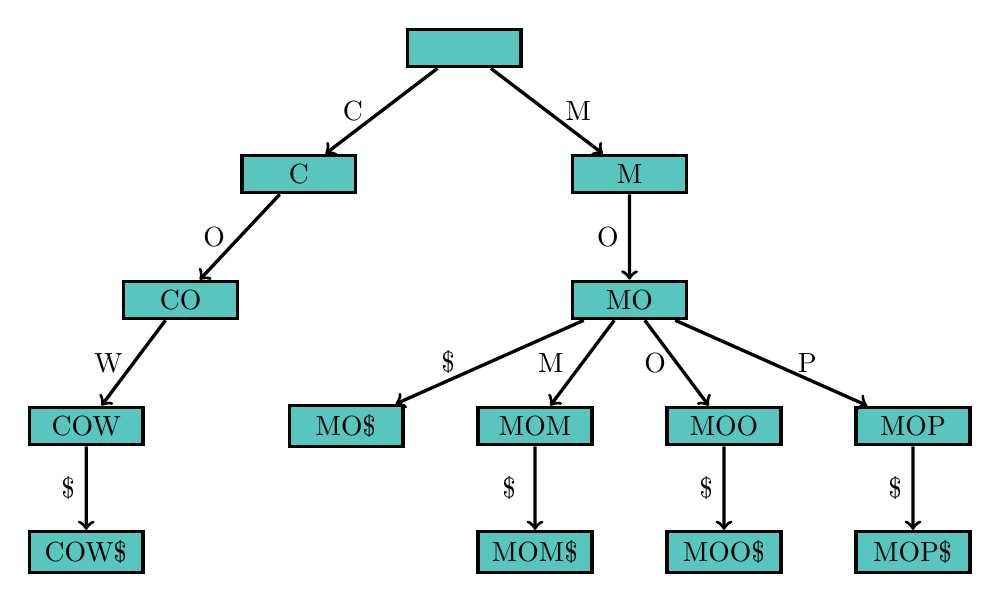
\begin{tikzpicture}[
  very thick,
  level 1/.style={sibling distance=42mm},
  level 2/.style={sibling distance=30mm},
  level 3/.style={sibling distance=24mm},
  level 4/.style={sibling distance=18mm},
  level distance=16mm,
  myrect/.style={
    draw,
    fill=myseagreen,
    text width=8ex,
    text centered
  }
]
\node [myrect] {\vphantom{A}}
child {
  node [myrect] {C}
  child {
    node [myrect] {CO}
    child {
      node [myrect] {COW}
      child {
        node [myrect] {COW\$}
        edge from parent [->] node [left] {\$}
      }
      edge from parent [->] node [left] {W}
    }
    child [missing]
    edge from parent [->] node [left, xshift=-0.5mm] {O}
  }
  child [missing]
  edge from parent [->] node [left, xshift=-1mm] {C}
}
child {
  node [myrect] {M}
  child {
    node [myrect] {MO}
    child {
      node [myrect] {MO\$}
      edge from parent [->] node [left, xshift=-3mm] {\$}
    }
    child {
      node [myrect] {MOM}
      child {
        node [myrect] {MOM\$}
        edge from parent [->] node [left, xshift=-1mm] {\$}
      }
      edge from parent [->] node [left, xshift=-1mm] {M}
    }
    child {
      node [myrect] {MOO}
      child {
        node [myrect] {MOO\$}
        edge from parent [->] node [left] {\$}
      }
      edge from parent [->] node [left] {O}
    }
    child {
      node [myrect] {MOP}
      child {
        node [myrect] {MOP\$}
        edge from parent [->] node [left] {\$}
      }
      edge from parent [->] node [right, xshift=2mm] {P}
    }
    edge from parent [->] node [left] {O}
  }
  edge from parent [->] node [right, xshift=1mm] {M}
}
;

\end{tikzpicture}
\end{center}

Insertion into a trie is straightfoward. We start at the root, and create edges and vertices as necessary until a path representing the string is formed. If a vertex already has an edge of the corect character leading out from it, we just travel down that edge. In order to identify the end of a string, we can append a ``\$'' to every string before we insert. Searching is the same as insertion, except we terminate our search when we can't go any further instead of adding a new edge. 

What we've seen so far doesn't make the trie seem particularly useful---string insertion and look up can be easily done in linear time with Rabin-Karp and a hash table as well. The advantage of the trie comes from its tree structure. Having common prefixes bundled together on the same path means we can compute compute information relating to prefixes easily. This allows for tree DPs that we wouldn't be able to do with hashing. (However, hashing does handle certain forms of prefix queries well, such as longest common prefix.)

Tries are also a building block for other string data structures, such as the Aho-Corasick automaton and the suffix tree. (In fact, tries can be viewed as a very simple form of string automaton.)

\section{Suffix Array}

For a string of length $n$, each index $i$ ($0 \le i < n$) can represent the suffix that starts at that index. A \emph{suffix array} is a list of these indices, sorted in lexicographically increasing order by suffix. Thus a suffix array is essentially a sorted list of the suffixes of a string. Below is the suffix array of ``mississippi\$.''

\begin{center}
  \begin{tabular}{r | l}
    Suffix Array & Suffix \phantom{moooooooooo} \\ \hline
    11 & \$ \\
    10 & i\$ \\
    7 & ippi\$ \\
    4 & issippi\$ \\
    1 & ississippi\$ \\
    0 & mississippi\$ \\
    9 & pi\$ \\
    8 & ppi\$ \\
    6 & sippi\$ \\
    3 & sissippi\$ \\
    5 & ssippi\$ \\
    2 & ssissippi\$ \\
  \end{tabular}
\end{center}

At first, it might seem surprising that such a structure is useful---why do we care about suffixes at all? The crucial observation is that every substring of a string is a prefix of a suffix. Thus if we have something that does well with prefixes, such as hashing or a trie, we use this to compute information about substrings. A trie built from suffixes is known as a \emph{suffix tree}, which we'll cover later. In this section, we'll go over what we can do with hashing and a suffix array.

First, let's figure out how we can construct a suffix array. The naive solution is to sort all $n$ suffixes using $O(n)$ string comparison. Since sorting itself takes $O(n \log n)$ comparisons, we have an $O(n^2 \log n)$ algorithm. However, with hashing and binary search, we can lexicographically compare two strings in $O(\log n)$ time. We do this by binary searching for the longest common prefix and then comparing the next character. We can can compute the hash of any substring with a polynomial hash, so it's easy to compare if the prefixes of two suffixes (a.k.a two substrings) are equal. Now that we have $O(\log n)$ comparison, our algorithm runs in $O(n \log^2 n)$ overall.

Note that it is also possible to compute suffix arrays in $O(n \log n)$ and even $O(n)$, but these algorithms are much more involved. For the purposes of contests, an $O(n \log^2 n)$ suffix array algorithm should almost always be enough.

With a suffix array, we can check if any queried ``needle'' string exists using a binary search with hashing. We can even count the number of occurences by binary searching for the first and last macth. This works in $O(m + \log n \log m)$, where $m$ is the length of the needle, because we need $O(\log m)$ operations for string comparison and $O(\log n)$ iterations of the binary search. Suffix arrays differ from KMP because KMP preprocesses the ``needle,'' while suffix arrays preprocess the ``haystack.'' 

From the suffix array, we can also obtain another useful data structure called the \emph{LCP array}. This array stores the longest common prefix between adjacent suffixes in the suffix array. We can use it to speed up pattern matching to $O(m + \log n)$. In addition, we can build a segment tree over the LCP array to answer queries, such as the LCP between two arbitrary suffixes.

Suffix arrays can also be used to solve many string problems beyond matching. This data structure does very well with most problems involving substrings. For example, suffix arrays/LCP arrays can count the number of distinct substrings in a string or return the $k$th lexicographically largest substring. The minimum string rotation problem can is another problem solvable with suffix arrays, since each rotation of a string $S$ is a substring of $S + S$.

To handle multiple strings with suffix arrays, we can either concatenate them with separator characters in between or separately compute their hashes.

Below is a short C++ code for computing suffix arrays. Look up lambda functions in C++ if you're not familiar with the syntax.

\begin{mylstlisting}[language=C++]
typedef unsigned long long ull;
// We use A as the exponent and M as the mod for our hash.
const ull M = 1000000007;
const ull A = 127;

void build(string S, int *sa){
  // Builds a suffix array for a string S in array sa.
  S.push_back('$');
  int N = S.size();
  ull P[N + 1], H[N + 1];
  P[0] = 1; // P stores the precomputed powers of A.
  H[0] = 0; // H stores the prefix hashes of S.
  for(int i = 0; i < N; i++){
    // Precomputing powers and hashes.
    P[i + 1] = A * P[i] % M;
    H[i + 1] = (A * H[i] + S[i]) % M;
    sa[i] = i;
  }
  auto f = [&](int a, int l){
    // Returns the hash of the substring starting at index a with length l.
    return (H[a + l] - H[a] * P[l] % M + M) % M;
  };
  auto comp = [&](int a, int b){
    // Compares the suffixes starting at indices a and b.
    int lo = 0, hi = min(N - a, N - b);
    while(lo + 1 < hi){
      int m = (lo + hi) / 2;
      (f(a, m) == f(b, m) ? lo : hi) = m;
    }
    return S[a + lo] < S[b + lo];
  };
  sort(sa, sa + N, comp);
}
\end{mylstlisting}

\section{Aho-Corasick}

One way to think about the Aho-Corasick algorithm is KMP/Z-algorithm on a trie. This algorithm is used for matching multiple needles in a single haystack and runs in time linear in the length of the haystack, with preprocessing linear in the total length of the needles. To do this, we first add all strings to a trie that stores some extra information at its nodes. Upon inserting each string, we mark the last node visited as a endpoint node. Each node, in addition to storing its children and its status as an endpoint node, stores a \emph{suffix link}. This link points to the longest proper suffix that is also a node on the trie. If necessary, each node can also store a \emph{dictionary suffix link}, which points to the first endpoint node reachable by only following suffix links.

To build an Aho-Corasick automaton, we start with a trie of the needle strings. What we want to do is compute the suffix links. We simplify this by using an $O(nk)$ approach, where $k$ is the alphabet size. For each node $n$, we compute an additional failure function, with one value corresponding to each letter of the alphabet. Suppose $p$ is the prefix represented by $n$. Then the failure function of $n$ for the letter $\alpha$ points to the node representing longest suffix of $p + \alpha$ in the trie.

We can compute all of this with a BFS. When we are at a node, we can find the suffix links of its children using the failure function of its own suffix link. We also have to calculate the node's own failure function. For every letter that has a corresponding child, its failure function is equal to that child. Otherwise, its failure function is equal to the corresponding failure function of the node's suffix link. Take a moment to think through why this works.

To query, we can iterate through our haystack string character by character and make the corresponding moves in the automaton. We follow the failure function when no child exists. However, note that there isn't really a distinction between a normal trie edge and a failed edge anymore. To check for matches, we can look at the values we store at each node and/or follow dictionary suffix links. To find all matches with dictionary suffix links, we have to follow the pointers until we reach a node that doesn't have a suffix in the dictionary. Note that if we follow dictionary suffix links, the complexity of our algorithm will also be linear in the number of matches. Here's an implementation of Aho-Corasick in C++ without dictionary suffix links:

\begin{mylstlisting}[language=C++]
const int SIGMA = 26;
const int MAXN = 100005;
// Each node is assigned an index where its data is stored.
// ch first stores the children of each node and later the failure function.
// val counts the number of strings ending at a given node.
// link stores suffix links.
int ch[MAXN][SIGMA], val[MAXN], link[MAXN], sz = 1;
// Array q is a hand-implemented queue.
// h and t point to the head and tail, respectively.
int q[MAXN], h, t;

void add(string s){
  // Adds a string to the trie.
  int p = 0; // p tracks our current position and starts at 0, the root.
  for(int i = 0; i < s.size(); i++){
    int c = s[i] - 'A';
    // ch[p][c] is 0 if null, so we have to allocate a new node/index.
    if(!ch[p][c]) ch[p][c] = sz++;
    p = ch[p][c];
  }
  val[p]++; // Updates endpoint marker.
}

void build(){
  // Computes all suffix links with a BFS, starting from the root.
  h = t = 0;
  q[t++] = 0;
  while(h < t){
    int v = q[h++], u = link[v];
    val[v] += val[u]; // Propagates endpoint marker.
    for(int c = 0; c < SIGMA; c++){
      if(ch[v][c]){
        // If child exists, we create a suffix link. 
        // The node's failure function here is the child.
        // Also, note that we have a special case if v is the root.
        link[ch[v][c]] = v ? ch[u][c] : 0;
        q[t++] = ch[v][c];
      } else {
        // Otherwise, we need to figure out its failure function.
        // We do this by using the failure function of the node's suffix link.
        ch[v][c] = ch[u][c];
      }
    }
  }
}
\end{mylstlisting}

\section{Advanced Suffix Data Structures}

I've yet to see these used in a contest, but they do exist. 

\subsection{Suffix Tree}

\subsection{Suffix Automaton}


\include{chapters/more_stuff}
\chapter{Math}

Algorithms here exhibit a different flavor than the graph theory, string, or geometry algorithms from earlier. This chapter is placed towards the end because material here doesn't really fit in any other section or the USACO canon, \textit{not} because this material is particularly difficult.

\section{Number Theory}

This section will contain much information about primes in many different ways. Indeed, prime numbers are the building blocks of number theory!

\subsection{Random Prime Numbers Bounds}

The point of this section is mostly to make the complexity analysis of the later sections easier. Therefore, I will list some useful theorems and bounds without proof. The proofs can be found in any standard number theory textbook or online. They are extremely insignificant in the context of the goals of this section.

\textbf{Prime Number Theorem}: The number of prime numbers less than $n$ is $O(\frac{n}{\log n})$ for any positive integer $n.$

\emph{Corollary}: The $n$-th prime number, $p_n$, is $O(n \log n).$

\textbf{Prime Number Harmonic Sum}: $\sum_{p \le n} \frac{1}{p} = O(\log \log n).$

\subsection{Prime Number Testing}

Let's say if you want to test is a number $n$ is prime. The most obvious way is to test all integers from $2$ to $n-1$, and see if they divide $n$. This takes $O(n)$ time. We can do better though! Note that if $n$ has a nontrivial factor, then it has one that is less than $\sqrt{n}.$ Indeed, if $n = pq,$ (as a nontrivial factorization) if both $p, q > \sqrt{n}$, then $pq > \sqrt{n}^2 = n$, a contradiction. So we only need to check whether $n$ has factors between $2$ and $\sqrt{n}.$ This takes $O(\sqrt{n})$ time. If you have precomputed a list of prime numbers (up to say $\sqrt{n}$), ten you only need to check whether $n$ has any prime factors in the same $2$ to $\sqrt{n}.$ This would give runtime $O(\frac{\sqrt{n}}{\log n})$ from the \emph{Prime Number Theorem} in section 10.1.1, a small but nontrivial improvement.

\subsection{Sieve of Eratosthenes}

If you want to compute all primes in the range $1$ to $n$. Runs in $O(n \log \log n)$. In other words, super fast.

\subsection{Prime Factorization}

How can we prime factorize a number? That is, given a positive integer $n$, how can we write it in the form $p_1 \cdot p_2 \cdot \dots \cdot p_k$, where the $p_i$ are all primes? Form example, $30 = 2 \cdot 3 \cdot 5$ and $24 = 2 \cdot 2 \cdot 2 \cdot 3$. The fact that every number can be uniquely factorized is called the \emph{Fundamental Theorem of Arithmetic}. Let's now figure out how to prime factorize every number efficiently. Using our intuition from above, we should expect that checking up to around $\sqrt{n}$ suffices. This is indeed true. The code below demonstrates:

\subsection{GCD and the Euclidean Algorithm}

I'll start once again with a theorem in number theory: if positive integers $a, b$ satisfy $\gcd(a, b) = 1$, then there exist integers $x, y$ such that $ax+by=1.$ This is called \emph{Bezout's Lemma.}

Similarly, if $\gcd(a, b) = g$, then there are integers $x, y$ such that $ax+by = g.$

%example gcd code here... and also some description of Euclidean Algorithm

\subsection{Fermat's Little Theorem}

Fermat's Little Theorem states that $a^p \equiv a \pmod{p}$ for any positive integer $a.$ Equivalently, we can say that $a^{p-1} \equiv 1 \pmod{p}.$

\subsection{Modular Inverses}

If $p$ is a prime, and $x$ satisfies $\gcd(x, p) = 1$, then there exists a positive integer $k$ such that $kx \equiv 1 \pmod{p}.$ $k$ is called the \emph{modular inverse} of $x \pmod{p},$ often just denoted as $1/x$ or $x^{-1}.$ Indeed, $1/x \cdot x = x^{-1} \cdot x = 1,$ so this notation is natural. The cool thing about modular inverses is that you can see them as division modulo $p.$ Since $x$ is nonzero $\pmod{p},$ it makes sense that you should be able to divide by $x.$ This is the main application of modular inverses. But how to find one quickly? There are two common algorithms, both of which run in $O(\log p)$ time. You can do this by running the Euclidean Algorithm described above: find positive integers $j, k$ such that $pj + kx = 1.$ Then obviously $kx \equiv 1 \pmod{p}.$ The other way is to notice that $x^{p-1} \equiv 1 \pmod{p}$ by Fermat's Little Theorem, so $x^{p-2} \equiv x^{-1} \pmod{p}.$ Now compute the left hand side of the previous expression using binary exponentiation.

Exercises related: Do $O(n \log p)$ precomputation to compute any binomial coefficient of the form $\binom{m}{k} \pmod{p}$ where $0 \le m, k \le n$ in $O(1)$ time.

\section{Combinatorial Games}

\url{https://activities.tjhsst.edu/sct/lectures/1314/impartial_games_12_06_13.pdf}

\section{Karatsuba}

\section{Matrices}

\section{Fast Fourier Transform}

\textit{This section generously contributed by Yang Liu.}

\subsection{Introduction}

The \emph{Fast Fourier Transform} (FFT) is a technique used to multiply two polynomials of degree $n$ in $O(n \cdot \log n)$ time. At a high level, what this algorithm is doing is something called \emph{polynomial interpolation}. This refers to the fact that if we know the value of a polynomial $P$ of degree $n$ at $n+1$ points, then we can uniquely determine the polynomial $P.$ The proof of this statement is simple, and involves the Lagrange Interpolation Formula for one direction and a simple root counting argument to prove uniqueness. I won't go into detail here because the proof isn't important, but it is useful to know some motivation behind the algorithm.

\subsection{Algorithm Outline}

Let's say we want to multiply 2 polynomials $A(x), B(x)$, both of degree $n$. Let $C(x) = A(x)B(x).$ The algorithm will proceed in 3 steps. Choose an integer $m > 2n,$ and choose $m$ numbers $x_0, x_1, \dots, x_{m-1}.$ I'll clarify what to choose $m$ and the $x_i$ as later. Just keep in mind that we can choose these values to be anything we want.

\begin{enumerate}

\item Evaluate $A(x_0), A(x_1), \dots, A(x_{m-1}).$ Similarly, evaluate $B(x_0), B(x_1), \dots, B(x_{m-1}).$

\item Evaluate $C(x_i) = A(x_i)B(x_i)$ for $0 \le i \le m-1.$

\item Interpolate the coefficients of $C(x)$ given the values $C(x_0), C(x_1), \dots, C(x_{m-1}).$

\end{enumerate}

The last step explains why we need $m > 2n.$ The degree of $C(x)$ is $2n$, so we need at least $2n+1$ points to determine $C(x)$ uniquely.

You should be skeptical that the above approach does any better than $O(n^2).$ In particular, step 1 seems like it should take $O(n^2).$ It turns out that if we choose the values $x_0, x_1, \dots, x_{m-1}$ properly, then we can do much better. Let me now describe what to choose $m$ to be, and what to choose $x_0, x_1, \dots, x_{m-1}$ to be.

\subsection{Roots of Unity}

Before telling you precisely, here's some food for thought. Let's take then example polynomial $A(x) = 1+2x+3x^2+4x^3+5x^4+6x^5+7x^6+8x^7.$ Let's split this into 2 groups: the even degree coefficients and odd degree coefficients. Let's call these two groups $A_{even}$ and $A_{odd}.$ Define $A_{even}(x) = 1+3x+5x^2+7x^3, A_{odd}(x) = 2+4x+6x^2+8x^7.$ Then clearly \[ A(x) = A_{even}(x^2) + x \cdot A_{odd}(x^2) \]

Notice that the $x^2$ in the formula makes it extremely easy to compute $A(-x)$ given $A(x).$ It's only one sign flip off! Therefore, it would be cool if our $x_i$ above were symmetric with respect to 0, i.e. if we want to compute $x$, we also should want to compute $-x$. An example set like this is $\{1, 2, 3, 4, -1, -2, -3, -4 \}.$ So if we wanted to compute $A(x)$ at these values, we would need to compute the values of $A_{even}, A_{odd}$ at their squares, that is $\{1, 4, 9, 16 \}.$ But this set is no longer symmetric! So this is not what we want exactly, since that means that we can't just recursively compute $A_{even}$ and $A_{odd}.$ So let's say that the set we want to compute $A_{even}, A_{odd}$ on is something like $\{1, 4, -1, -4 \}.$ Then the values that we get for $A(x)$ are $\{1, -1, 2, -2, i, -i, 2i, -2i \}.$ Complex numbers! This is closer to what we want, but still not precisely. The selection of the $x_i$ explained below makes everything work out perfectly.

So what should we choose $m$ and the $x_i$ to be? I'll tell you now and then explain why this selection works so well: choose $m$ to be a power of $2$ that is larger than $2n$, and choose $x_0, x_1, \dots, x_{m-1}$ to be the $m$\emph{-th roots of unity}. The $m$-th roots of unity are complex numbers that satisfy the equation $x^m = 1.$ They are of the form $\cos\left(\frac{2k\pi i}{m}\right) + i \cdot \sin\left(\frac{2k\pi i}{m} \right)$ for any integer $k$ from $0$ to $m-1.$

Let $\omega$ be a \emph{primitive} root of unity, i.e. the smallest $m'$ such that $\omega^{m'} = 1$ is $m' = m.$ We can without loss of generality set $\omega = \cos\left(\frac{2\pi i}{m}\right) + i \cdot \sin\left(\frac{2\pi i}{m} \right).$ One can easily check the the remaining roots of unity are $\omega^2, \omega^3, \dots, \omega^m.$ From now on, let's just set $x_i = \omega^i$ for all $0 \le i \le m-1.$ Note that $x_0 = 1.$ Also set $m = 2^k > 2n.$ Now I can proceed to describing why this algorithm works.

\subsection{Algorithm Specifics: Step 1}

In this section I'll implement (using pseudocode) a function 

vector<double> fft(vector<int> $A$, k, $\omega$). This means that this will return a vector<double> of length $2^k$ containing the values $A(\omega^0), A(\omega^1), A(\omega^2), \dots, A(\omega^{2^k-1}).$ Remember that $\omega^{2^k} = 1.$ The vector<int> $A$ stores the coefficients of $A(x)$. The $x^i$ coefficient of $A$ would be stored as $A[i].$

Here's an implementation. The brackets $\{ \}$ will be shorthand for containing a vector.

\begin{algorithm}[H]
\caption{FFT}
%\label{}
\begin{algorithmic}
\Function{fft}{vector<int> $A, k, \omega$} \Comment $\omega^{2^k} = 1$
	\State $A$.resize($2^k$)
	\State vector<double> $f, f_{even}, f_{odd}$
	\State $f$.resize($2^k$)
	
	\If {$k = 0$}
		\State \Return $ \{A[0] \}$ \Comment a vector of length 1
    \EndIf
    \State $A_{even}$ = $ \{A[0], A[2], \dots, A[2^k-2] \}$
    \State $A_{odd}$ = $ \{A[1], A[3], \dots, A[2^k-1] \}$
    \State $f_{even} = $ \Call{fft}{$A_{even}, k-1, \omega^2$}
    \State $f_{odd} = $ \Call{fft}{$A_{odd}, k-1, \omega^2$}
    
    \ForAll {$i = 0, i < 2^{k-1}, i++$}
    	\State $f[i] = f_{even}[i] + \omega^i \cdot f_{odd}[i]$
	\State $f[i+2^{k-1}] = f_{even}[i] - \omega^i \cdot f_{odd}[i]$

	\EndFor

\Return f

\EndFunction

\end{algorithmic}
\end{algorithm}

So why does this algorithm work? Note that the algorithm proceeds recursively, calling itself twice (once for even, once for odd). $A_{even}(x)$ is the polynomial $A[0] + A[2]x + A[4]x^2 + \dots + A[2^k-2]x^{2^{k-1}-1}.$ Therefore, what the recursive call is doing is computing the values of $A_{even}$ at the values $x = \omega^0, \omega^2, \omega^4, \dots, \omega^{2^k-2}.$ This is equivalent to computing the values of the polynomial $B_{even}(x) = A[0] + A[2]x^2 + A[4]x^4 + \dots + A[2^k-2]x^{2^{k}-2}$ at the values $x = \omega^0, \omega^1, \omega^2, \dots, \omega^{2^{k-1}-1}.$ The recursive call for $A_{odd}(x) = A[1] + A[3]x + A[5]x^2 + \dots + A[2^k-1]x^{2^{k-1}-1}$ behaves in a similar way. Similarly, define $B_{odd}(x) = A[1] + A[3]x^2 + A[5]x^4 + \dots + A[2^k-1]x^{2^{k}-2}.$

The key is to note that $A(x) = B_{even}(x) + x \cdot B_{odd}(x).$ Since we know the values of $B_{even}(x), B_{odd}(x)$ for $x = \omega^0, \omega^1, \dots, \omega^{2^{k-1}-1},$ we also can compute the values of $A(x)$ for these values of $x$. But what about the remaining values? This requires the observation that $\omega^{i + 2^{k-1}} = -\omega^i.$ Since $B_{even}(x), B_{odd}(x)$ only have even powers, $B_{even}(\omega^i) = B_{even}(-\omega^i) = B_{even}(\omega^{i + 2^{k-1}}).$ The same equality also holds for $B_{odd}(x).$ Using this observation along with the equation $A(x) = B_{even}(x) + x \cdot B_{odd}(x),$ we can see now why the two equations in the for loop of the code above hold. And that's how we do Step 1!

Let's analyze the runtime of this function FFT. Let $T(2^k)$ denote the time needed to run FFT on an array of length $2^k.$ Then $T(2^k) = 2T(2^{k-1}) + O(2^k) \implies T(2^k) = k \cdot 2^k,$ by the Master Theorem. Since $2^k$ is $O(n)$ by the above discussion, this steps runs in $O(n \cdot \log n)$ time.

\subsection{Algorithm Specifics: Step 2}

I'll give you a rest after a hard theoretical previous section. You do this step by looping through the values $A(x_0), A(x_1), \dots, A(x_{2^k-1}), B(x_0), B(x_1), \dots, B(x_{2^k-1})$ and directly multiplying $C(x_i) = A(x_i)B(x_i).$ This step runs in $O(n)$ time.

\subsection{Algorithm Specifics: Step 3}

This may seem like something completely new, but actually most of the work is already done. I'll explain. In fact I claim that writing the code $C = \text{fft}(C, k, \omega^{-1}),$ and then dividing all elements of $C$ by $2^k$ finishes. You should believe me on this. If you work out the computations, you'll see that this is true. You can think of it kind of as a roots of unity filter if you know what that means. If not, just be happy that step 3 is very easy once you have Step 1!

\subsection{A Brief Note on Number Theory}

There is a slight variation on FTT that avoids using complex numbers completely. Complex numbers are often bad at precision and run slowly. There is a way to make FFT work over only the integers, which is pretty cool. Here's a brief description how.

We work $\pmod{p}$ for a suitable prime $p$. The reason we need $p$ to be prime is so that division works as we want. As explained in the above section on number theory, every nonzero number modulo $p$ has a unique inverse, so division works as expected. There are also integers $g$ such that $g^0, g^1, \dots, g^{p-2}$ run through all nonzero numbers $\pmod{p}.$ These are called \emph{primitive roots}. This means that modulo $p$ behaves a whole lot like the roots of unity that we want. More specifically, we want an integer $\omega$ such that the smallest integer $m$ that satisfies $\omega^m = 1$ is $m = 2^k,$ for some power of $2.$ So when can we find such an $\omega?$ By the discussion of primitive roots, this can happen precisely when $2^k | p-1.$ Then all we do is find a primitive root $g$, and take $\omega = g^{\frac{p-1}{2^k}}.$ Finding primitive roots is fast because math proves that there is always a small primitive root. So everything works just as you expect! The same exact code works, just put a $\pmod{p}$ at the end of every line and you're set.

\appendix

\listofalgorithms

\end{document}
